\newcommand{\bom}{\perp}  % bottom _|_
\newcommand{\al}{\prec}
\newcommand{\tAL}{\textsf{transAL}}
\newcommand{\Sbasis}{\mathcal{S}}  % standard basis
\newcommand{\Tbasis}{\mathcal{L}}  % linear basis
\newcommand{\lmul}[1]{{}_{#1}*}  % left multiplication node
\newcommand{\rmul}[1]{*_{#1}}  % right multiplication node
\newcommand{\op}{\mathrm{op}}  % opposite
\newcommand{\RMod}[1]{#1\text{\sf-Mod}}  % The category of left R-modules
\newcommand{\ModR}[1]{\text{\sf Mod-}#1}  % The category of right R-modules
\newcommand{\pspace}{\mathcal{P}}  % the parameter space
\newcommand{\s}{\underline}
\renewcommand{\l}{\overline}


\lstset{
  upquote=true,
  basicstyle=\ttfamily\small,          % print whole listing in typewriter
  keywordstyle=\color{blue}\bfseries, % bold blue keywords
  %identifierstyle=,           % nothing happens
  commentstyle=\color{green}, % green comments
  stringstyle=\color{red},      % typewriter type for strings
  showstringspaces=false     % no special string spaces
}


\part{The transposition principle}

The complexity of algebraic algorithms is often more easily described
in a non-Turing model where one assumes that any algebraic operation
can be done in a unit of time and any other operation is
free. \emph{Algebraic complexity} studies precisely the computational
models that behave this way.

For algorithms over finite rings, the algebraic complexity gives a
precise estimate for the complexity in the Turing model (also called
the \emph{binary complexity}). For other rings, the algebraic estimate
may be way off target, but it can nevertheless give useful information.

In this chapter we study models that allow one to study the algebraic
complexity of linear operators. We first present the \emph{arithmetic
  circuit}, then the \emph{straight line program}. Because of their
algebraic structure, these models support some algebraic
manipulations.  Our principal interest will be the \emph{transposition
  theorem}, stating that it is possible to apply classical duality (in
the sense of Section~\ref{sec:linear-algebra:duality}) to programs,
while preserving some complexity invariants. The interest for the
transposition theorem comes from the applications we have seen in
Section~\ref{sec:transp-algor} and other more advanced applications
that we will see in the next chapters.

Finally, in Section~\ref{sec:word-about-automatic}, we study the
relationship between the transposition theorem and the classical
theory of \emph{automatic differentiation}.



% Local Variables:
% mode:flyspell
% ispell-local-dictionary:"american"
% mode:reftex
% mode:TeX-PDF
% TeX-master: "../these"
% End:
%

\section{\index{arithmetic circuit}Arithmetic circuits}
\label{sec:circuits}

In this section we present the arithmetic circuit model and give some
classical results. Since we have in mind applications to the theory of
transposition, our presentation is slightly different from classical
presentations of the subject \cite{BuClSh, Vollmer}.

\begin{definition}[Arithmetic operator, arity]
  Let $R$ be a (non necessarily commutative) ring with unit. An
  arithmetic operator over $R$ is a function $f:R^i\ra R^o$ for some
  $i,o\in\N$.  Here $i$ is called the \emph{in-arity} of $f$ or simply
  \emph{arity}, $o$ is called the \emph{out-arity} of $f$.
\end{definition}

The exact meaning of the product $R^n$ varies depending on what is
meant by ``function'': a category must be specified in order for this
notions to be well defined. In this paper we will use two different
definitions:
\begin{itemize}
\item If we want ``function'' to mean any function in a set-theoretic
  sense, we work in the category $\mathsf{Set}$. Then $R^n$ is the
  product $\prod^nR$ of the category (the Cartesian product) and $R^0$
  is the terminal object of the category, i.e. any singleton. For
  convenience we note $\{\bom\}$ for $R^0$, with $\bom$ being its
  unique element.
\item In some cases it will be convenient to restrict ``function'' to
  mean ``morphism of left $R$-modules'', then we will work in the
  category $\RMod{R}$ of left $R$-modules with morphisms. Then $R^n$
  is the product $\prod^nR$ of the category and $R^0$ is the zero
  module.  We note $0$ for the zero module and $\bom$ for its unique
  element in order to avoid confusion with the $0$ of $R$ (and to
  stress the analogy with $\mathsf{Set}$). In what follows by
  ``module'' we will always mean ``left module''.
\end{itemize}

\begin{definition}[Arithmetic basis]
  Let $R$ be a ring.  An arithmetic $R$-basis is a (not necessarily
  finite) set of arithmetic operators over $R$.
\end{definition}

Two arithmetic bases will be important to us. The first one is the
\emph{standard basis}, noted $\Sbasis$. It is composed of the
following operators
\begin{equation}
  \label{eq:sbasis}
  \tag{$\Sbasis$}
  \begin{aligned}
    + : R\times R &\ra R    & * : R\times R &\ra R &  \hub : R &\ra R\times R\\
        a, b &\mapsto a+b   &     a, b &\mapsto ab &         a &\mapsto a,a\\ \\
    \eta_a : \{\bom\} &\ra R     &&& \omega : R &\ra \{\bom\} \\
          \bom &\mapsto a &&&          a &\mapsto \bom
  \end{aligned}
\end{equation}
Remark that $\eta_a$ defines a possibly infinite family of operators,
one for every $a\in R$.

The other one is the \emph{linear basis}, noted $\Tbasis$.  It
is composed of
\begin{equation*}
  \label{eq:tbasis}
  \tag{$\Tbasis$}
  \begin{aligned}
    + : R\times R &\ra R    &\quad
    \rmul{a} : R &\ra R      &\quad
    0 : 0 &\ra R  \\
    a, b &\mapsto a+b   &
    b &\mapsto ba &  
    \bom &\mapsto 0  \\
    \\
    \hub : R &\ra R\times R  &\quad
    &&
    \omega : R &\ra 0 \\
    a &\mapsto a,a    &
    &&
    a &\mapsto \bom
  \end{aligned}
\end{equation*}
The linear basis is reproduced in figure \ref{fig:nodes}.

Finally, the \emph{opposite linear basis}, noted $\Tbasis^\op$, is
obtained from $\Tbasis$ by substituting $\rmul{a}$ with
$\lmul{a}:b\mapsto ab$. Notice that this is just a shorthand notation
for the arithmetic $R^\op$-basis $\Tbasis$.

In terms of category theory, $\Sbasis$ only makes sense when working
with $\mathsf{Set}$, while $\Tbasis$ can be defined even when working
with $\RMod{R}$ (equivalently, $\Tbasis^\op$ can be defined when
working with $\ModR{R}$, the category of right $R$-modules).
\begin{figure}[!ht]
  \label{fig:nodes}
  \centering
  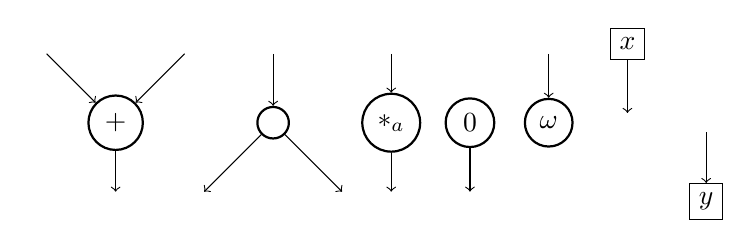
\begin{tikzpicture}
    \tikzstyle{node}=[circle,thick,draw=black,minimum size=4mm]
    \tikzstyle{arg}=[rectangle,thin,draw=black,minimum size=4mm]
    
    \begin{scope}
      \node(in1){};
      \node(nop)[right of=in1]{};
      \node(in2)[right of=nop]{};

      \node[node](plus)[below of=nop]{$+$};
      \node(out)[below of=plus]{};

      \path[->]
      (in1) edge (plus)
      (in2) edge (plus)
      (plus) edge (out);
    \end{scope}
    
    \begin{scope}[xshift=30mm]
      \node(in){};
      \node[node](hub)[below of=in]{$\hub$};
      \node(nop)[below of=hub]{};
      \node(out1)[left of=nop]{};
      \node(out2)[right of=nop]{};

      \path[->]
      (in) edge (hub)
      (hub) edge (out1)
      (hub) edge (out2);
    \end{scope}
    
    \begin{scope}[xshift=45mm]
      \node(in){};
      \node[node](times)[below of=in]{$\rmul{a}$};
      \node(out)[below of=times]{};

      \path[->]
      (in) edge (times)
      (times) edge (out);
    \end{scope}

    \begin{scope}[xshift=55mm]
      \node(nop){};
      \node[node][below of=nop](create){$0$};
      \node(out)[below of=create]{};
      \path[->] (create) edge (out);
    \end{scope}

    \begin{scope}[xshift=65mm]
      \node(in){};
      \node[node][below of=in](destroy){$\omega$};
      \node(nop)[below of=destroy]{};
      \path[->] (in) edge (destroy);
    \end{scope}

    \begin{scope}[xshift=75mm]
      \node[arg](in){$x$};
      \node[below of=in](out){};
      \path[->] (in) edge (out);
    \end{scope}

    \begin{scope}[xshift=85mm]
      \node(nop){};
      \node[below of=nop](in){};
      \node[arg](out)[below of=in]{$y$};
      \path[->] (in) edge (out);
    \end{scope}
  \end{tikzpicture}
  \caption{Nodes over the linear basis: round ones are evaluation
    nodes, square ones are input and output nodes.}
\end{figure}


Arithmetic circuits are directed acyclic multigraphs carrying
information from an arithmetic basis; the formal definition follows.

\begin{definition}[Arithmetic node]
  Let $R$ be a ring and $\mathcal{B}$ be an $R$-basis. A node over
  $(R,\mathcal{B})$ is a tuple $v=(I, O, f)$ such that
  \begin{itemize}
  \item $I$ and $O$ are finite ordered sets, 
  \item $f$ is either an element of $\mathcal{B}$ or the special value
    $\emptyset$.
  \item If $f=\emptyset$, one of the two following conditions must hold:
    \begin{itemize}
    \item $I$ is a singleton and $O$ is empty, in this case we say
      that $v$ is an \emph{input node};
    \item $I$ is empty and $O$ is a singleton, in this case we say
      that $v$ is an \emph{output node}.
    \end{itemize}
  \item If $f\ne\emptyset$, the cardinality of $I$ matches the
    in-arity of $f$ and the cardinality of $O$ matches the out-arity
    of $f$; in this case we say that $v$ is an \emph{evaluation node}.
  \end{itemize}
\end{definition}

We call \emph{input ports} the elements of $I$ and \emph{output ports}
the elements of $O$, we note respectively $\inp(v)$ and
$\outp(v)$. The cardinalities of $I$ and $O$ are called, respectively,
the \emph{in-degree} and \emph{out-degree} of $v$.  We call $f$ the
value of $v$ and note $\beta(v)$.

\begin{definition}[Arithmetic circuit]
  Let $R$ be a ring and $\mathcal{B}$ be an $R$-basis. An arithmetic
  circuit over $(R,\mathcal{B})$ is a tuple $C=(V,E)$ such that
  \begin{enumerate}
  \item $V$ is a finite ordered set of nodes over $(R,\mathcal{B})$,
  \item let $I=\biguplus_{v\in V}\inp(v)$ and $O=\biguplus_{v\in
      V}\outp(v)$, then $E$ is a bijection from $O$ to $I$.
  \end{enumerate}
\end{definition}

It is useful to see $E$ as a set of pairs $(o,i)$ with $i\in I$ and
$o\in O$. Then the elements of $E$ are called the \emph{edges} of the
circuit. The edges \emph{incident} to $v\in V$ are all the $(o,i)\in
E$ such that $i\in\inp(v)$; the edges \emph{stemming} from $v\in V$
are all the $(i,o)\in E$ such that $o\in\outp(v)$. An edge stemming
from $v$ and incident to $v'$ is said to \emph{connect} $v$ to $v'$.
We call \emph{inputs} and \emph{outputs} of a circuit, respectively,
the input and output nodes in $V$; we note $\inp(C)$ and $\outp(C)$.

By forgetting the ordering of $V$, a circuit induces a multiDAG with
labelled nodes, we call it the \emph{graph} of $C$. In what follows we
will often refer to graph-theoretic properties of the graph without
explicitly making the difference between a circuit and its graph.

Figure \ref{fig:circuit} shows an example of arithmetic circuit, the
analogy with multiDAGs is evident. We draw input and output nodes in
square boxes and evaluation nodes in round boxes. The orders on input
and output ports are implicitly represented by ordering edges
clockwise starting from 9 on the clock. The order on $V$ is actually
only important for input and output nodes: we implicitly represent
this information by arranging input and output nodes increasingly from
left to right, but we omit it for evaluation nodes. We will always use
these conventions when drawing circuits.

\begin{figure}[!ht] \centering
  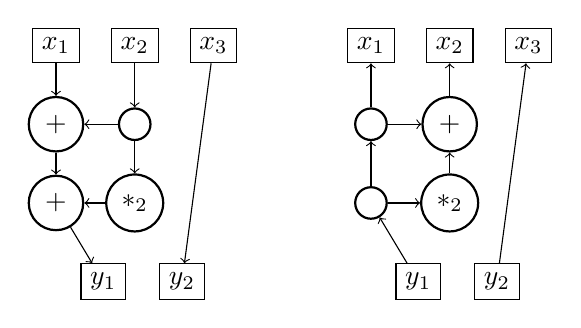
\begin{tikzpicture}
\tikzstyle{node}=[circle,thick,draw=black,minimum size=4mm]
\tikzstyle{arg}=[rectangle,thin,draw=black,minimum size=4mm]
    
    \begin{scope} \node[arg](in1){$x_1$}; \node[arg,right
of=in1](in2){$x_2$}; \node[arg,right of=in2](in3){$x_3$};
      
      \node[node,below of=in1](plus1){$+$}; \node[node,right
of=plus1](H){$\hub$};

      \node[node,below of=plus1](plus2){$+$}; \node[node,right
of=plus2](times){$*_2$};

      \node[arg,below of=plus2,xshift=6mm](out1){$y_1$};
\node[arg,right of=out1](out2){$y_2$};

      \path[->] (in1) edge (plus1) (in2) edge (H) (in3) edge (out2)
(H) edge (plus1) (H) edge (times) (plus1) edge (plus2) (times) edge
(plus2) (plus2) edge (out1);
    \end{scope}

    \begin{scope}[xshift=4cm]
      \node[arg](in1){$\dual{x_1}$};
      \node[arg,right of=in1](in2){$\dual{x_2}$};
      \node[arg,right of=in2](in3){$\dual{x_3}$};
      
      \node[node,below of=in1](plus1){$\hub$};
      \node[node,right of=plus1](H){$+$};

      \node[node,below of=plus1](plus2){$\hub$};
      \node[node,right of=plus2](times){$*_2$};

      \node[arg,below of=plus2,xshift=6mm](out1){$\dual{y_1}$};
      \node[arg,right of=out1](out2){$\dual{y_2}$};

      \path[<-]
      (in1) edge (plus1)
      (in2) edge (H)
      (in3) edge (out2)
      (H) edge (plus1)
      (H) edge (times) 
      (plus1) edge (plus2)
      (times) edge (plus2)
      (plus2) edge (out1);
    \end{scope}
  \end{tikzpicture}
  \caption{Two arithmetic circuits over $\Tbasis$. The linear map
    $y_1=x_1+3x_2, y_2=x_3$ is computed by the circuit on the left and
    its transpose is computed by the circuit on the right.}
  \label{fig:circuit}
\end{figure}

Circuits would be meaningless if they hadn't a semantic attached to
them. Intuitively the semantic corresponds to evaluation of the nodes
along the flow of the multiDAG.

\begin{definition}[Evaluation of an arithmetic circuit]
  \label{def:eval}
  Let $C$ be an arithmetic circuit with $i$ inputs and $o$ outputs,
  then its evaluation is a function $\eval_C:R^i\ra R^o$.

  In order to define it, we simultaneously define the evaluation
  $\eval_v$ of each $v\in V$ and the evaluation $\eval_e$ of each
  $e\in E$. We will note by $<_v$ the orders on the input and the
  output ports of $v$; we will also note by $<_V$ the order on $V$.
  \begin{itemize}
  \item Let $v\in V$ have out-degree $n$, let its evaluation be
    $\eval_v:R^i\ra R^n$ and let $\pi_1,\ldots,\pi_n$ be the canonical
    projections from $R^n$ to $R$. Let $o_1<_v\cdots<_vo_n$ be the
    output ports of $v$ and let $e_j=\bigl(o_j,E(o_j)\bigr)$ be the
    corresponding edges stemming from $v$, then $\eval_{e_j} =
    \pi_j\circ\eval_v$ for any $j$.
  \item Let $x_1<_V\cdots<_Vx_n$ be the input nodes and let
    $\pi_1,\ldots,\pi_i$ be the canonical projections from $R^i$ to
    $R$, then $\eval_{x_j}=\pi_j$ for any $j$.
  \item For every evaluation node $v$ with in-degree $m$, let
    $i_1<_v\cdots<_vi_m$ be the input ports of $v$ and let
    $e_j=\bigl(E^{-1}(i_j),i_j\bigr)$ be the corresponding edges
    incident to $v$, then
    \begin{equation}
      \label{eq:eval_v}
      \eval_v = \beta(v) \circ (\eval_{e_1} \times \cdots \times \eval_{e_m})
      \text{.}
    \end{equation}
  \item For every output node $y$, let $e\in E$ be the only edge
    incident to $y$, then $\eval_y=\eval_e$.
  \end{itemize}

  We can finally define $\eval_C:R^i\ra R^o$. Let $y_1<_V\cdots<_Vy_o$
  be the output nodes, then
  \begin{equation}
    \label{eq:eval}
    \eval_C = \eval_{y_1} \times \cdots \times \eval_{y_o}
    \text{.}
  \end{equation}
  We also say that $C$ \emph{computes} $\eval_C$.
\end{definition}

Observe that the products of functions in equation \eqref{eq:eval_v}
and \eqref{eq:eval} are formally defined via the universal property of
the product: for any collection of functions $f_j:X\ra R$, the product
$f=\prod_jf_j$ is the unique function $f:X\ra \prod_jR$ such that
$f_j=\pi_j\circ f$ for any $j$. This allows us to easily show the
following property.

\begin{proposition}
  The evaluation of an arithmetic circuit is an arrow (a function) in
  the category of interest. In particular, the evaluation of a circuit
  over $(R,\Tbasis)$ is a morphism of $R$-modules.
\end{proposition}

The converse is not necessarily true : not any arrow of the category
can be computed by a circuit. However for the basis $\Tbasis$ it is
possible to give a partial converse.

\begin{proposition}
  Any morphism of free finite-dimensional $R$-modules can be computed
  by an arithmetic circuit over $(R,\Tbasis)$.
\end{proposition}
\begin{proof}
  Take the matrix associated to such morphism and create a circuit
  that performs the matrix-vector product.
\end{proof}

Circuits can be composed in a natural way by connecting their inputs
and outputs.

\begin{definition}[Composition of circuits]
  Let $C=(V,E)$ and $C'=(V',E')$ be two circuits over
  $(R,\mathcal{B})$ and let $\mathcal{R}:\outp(C)\ra\inp(C')$ be an injective
  partial function. The composition of $C$ and $C'$ through
  $\mathcal{R}$, noted $C'\overset{\mathcal{R}}{\circ}C$, is the
  circuit $(V'', E'')$ such that
  \begin{itemize}
  \item $V'' = \bigr(V - \mathcal{R}^{-1}(\inp(C'))\bigr) \uplus
    \bigl(V' - \mathcal{R}(\outp(C))\bigr)$ with the orders inherited
    from $V$ and $V'$ and the supplementary condition that $v<v'$
    whenever $v\in V$ and $v'\in V'$.
  \item $E''(o) = \begin{cases}
      E'(o') & \text{if $E(o)\in\inp(v')$ and $\mathcal{R}(v') = v''$ and $\outp(v'')=\{o'\}$,}\\
      (E\uplus E')(o) & \text{otherwise.}
    \end{cases}$
  \end{itemize}

  When the function $\mathcal{R}$ is total, bijective and monotone
  (w.r.t. the orders on $V$ and $V'$), we say the the composition is
  \emph{natural} and simply note $C'\circ C$.
\end{definition}


\begin{figure}[!ht] \centering
  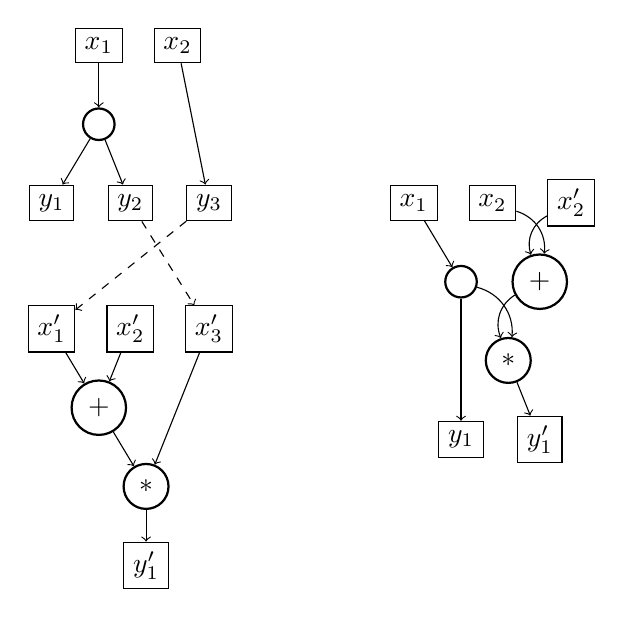
\begin{tikzpicture}
    \tikzstyle{node}=[circle,thick,draw=black,minimum size=4mm]
    \tikzstyle{arg}=[rectangle,thin,draw=black,minimum size=4mm]
    
    \begin{scope}
      \node[arg](in1){$x_1$};
      \node[arg,right of=in1](in2){$x_2$};
      
      \node[node,below of=in1](H){$\hub$};

      \node[arg,below of=H, xshift=-6mm](out1){$y_1$};
      \node[arg,right of=out1](out2){$y_2$};
      \node[arg,right of=out2](out3){$y_3$};

      \path[->]
      (in1) edge (H)
      (in2) edge (out3)
      (H) edge (out1)
      (H) edge (out2);

      \node[arg,below of=out1,yshift=-6mm](in3){$x'_1$};
      \node[arg,right of=in3](in4){$x'_2$};
      \node[arg,right of=in4](in5){$x'_3$};

      \node[node,below of=in3,xshift=6mm](plus1){$+$};
      
      \node[node,below of=plus1,xshift=6mm](plus2){$*$};

      \node[arg,below of=plus2](out4){$y'_1$};

      \path[->]
      (in3) edge (plus1)
      (in4) edge (plus1)
      (plus1) edge (plus2)
      (in5) edge (plus2)
      (plus2) edge (out4);

      \path[->,dashed]
      (out2) edge (in5)
      (out3) edge (in3);
    \end{scope}

    \begin{scope}[xshift=3cm,yshift=-3cm]
      \Large
      \node(=>){$\Ra$};
    \end{scope}

    \begin{scope}[xshift=4cm,yshift=-2cm]
      \node[arg](in1){$x_1$};
      \node[arg,right of=in1](in2){$x_2$};
      \node[arg,right of=in2](in4){$x'_2$};
      
      \node[node,below of=in1,xshift=6mm](H){$\hub$};

      \node[node,below of=in2,xshift=6mm](plus1){$+$};
      
      \node[node,below of=plus1, xshift=-4mm](plus2){$*$};

      \node[arg,below of=plus2,xshift=4mm](out4){$y'_1$};
      \node[arg,left of=out4](out1){$y_1$};

      \path[->]
      (in1) edge (H)
      (in2) edge[bend left=40] (plus1)
      (H) edge[bend left=40] (plus2)
      (H) edge (out1);

      \path[->]
      (in4) edge[bend right=40] (plus1)
      (plus1) edge[bend right=40] (plus2)
      (plus2) edge (out4);
    \end{scope}
  \end{tikzpicture}
  \caption{Composition of circuits through $\mathcal{R} = \{y_2\mapsto
    x'_3, y_3\mapsto x'_1\}$.}
  \label{fig:composition}
\end{figure}
An example of composition is given in figure \ref{fig:composition}.
It is evident that the concept of natural composition coincides with
composition of functions, the proof of the following proposition is
trivial.

\begin{proposition}
  Let $C$ and $C'$ be circuits over $(R,\mathcal{B})$ and let $C$
  have as many outputs as $C'$ has inputs, then
  \[\eval_{C'\circ C} = \eval_{C'}\circ\eval_{C} \text{.}\]
\end{proposition}

Another evidence that we state without proof is the fact that any
circuit over $(R,\mathcal{B})$ can be obtained by composition of small
elementary circuits.

\begin{proposition}
  We call \emph{elementary} a circuit that has one unique evaluation
  node. Any circuit can be obtained by composition of elementary
  circuits.
\end{proposition}

We finally define a way of substituting nodes, first syntactically,
then semantically.

\begin{definition}[Syntactic substitution]
  Let $C=(V,E)$ be a circuit over $(R,\mathcal{B})$ and let
  $C'=(V',E')$ be a circuit over $(R,\mathcal{B}')$. Let $C'$ have $i$
  inputs and $o$ outputs and let $v\in V$ have in-degree $i$ and
  out-degree $o$. 

  Let $\mathcal{I}$ and $\mathcal{O}$ be monotone bijections
  respectively from $\inp(v)$ to $\inp(C')$ and from $\outp(C')$ to
  $\outp(v)$. We note by $C[C'/v]$ the circuit $(V'',E'')$ over
  $(R,\mathcal{B}\cup\mathcal{B}')$ defined as follows:
  \begin{itemize}
  \item $V'' = V\uplus (V' - \inp(C') - \outp(C'))$,
  \item $E''(o) = \begin{cases}
      E'(o') & \text{if $E(o)\in\inp(v)$ and $\mathcal{I}(E(o))=v'$ and $\outp(v')=\{o'\}$,}\\
      E(o') & \text{if $E'(o)\in\outp(C')$ and $\mathcal{O}(E'(o))=o'$,}\\
      (E\uplus E')(o) & \text{otherwise.}
    \end{cases}$
  \end{itemize}
\end{definition}

\begin{definition}[Semantic substitution]
  Let $C$ be a circuit over $(R,\mathcal{B}\cup\{f\})$ and let $F$ be
  a circuit over $(R,\mathcal{B})$ such that $\eval_F=f$.

  We note by $C[F/f]$ the circuit over $(R,\mathcal{B})$ where any
  node $v$ of $C$ such that $\beta(v)=f$ has been syntactically
  substituted by $F$.

  It is obvious that
  \[\eval_{C[F/f]} = \eval_C \text{.}\]
\end{definition}

As a shorthand notation, we will draw octogones to signify that a node
has been syntactically substituted by a circuit, without giving the
actual shape of the substituting circuit. Figure
\ref{fig:substitution} shows an example.

\begin{figure}[!ht]
  \label{fig:substitution}
  \centering
  \begin{tikzpicture}
    \tikzstyle{node}=[circle,thick,draw=black,minimum size=4mm]
    \tikzstyle{arg}=[rectangle,thin,draw=black,minimum size=4mm]
    \tikzstyle{subst}=[regular polygon,regular polygon sides=8,thick,draw=black,minimum size=4mm]
    
    \begin{scope}
      \node[arg](in1){$x_1$};
      \node[arg,right of=in1](in2){$x_2$};
      
      \node[node](H)[below of=in2]{$\hub$};
      \node[subst](F)[left of=H]{$F$};

      \node[arg,below of=F,xshift=-6mm](out1){$y_1$};
      \node[arg,right of=out1](out2){$y_2$};
      \node[arg,right of=out2](out3){$y_3$};

      \path[->]
      (in1) edge (F)
      (in2) edge (H)
      (H) edge[bend left=10] (F)
      (H) edge[bend right=10] (F)
      (F) edge (out1)
      (F) edge (out2)
      (F) edge (out3);
    \end{scope}

  \end{tikzpicture}
  \caption{Arithmetic circuit where a node has been syntactically
    substituted by a circuit $F$ with $3$ inputs and $3$ outputs.}
\end{figure}

This shows that circuits are a good formalism to describe
functions. However, they carry more information than simply their
evaluation; the next step is to classify them in a
complexity-theoretic way.

\begin{definition}[Size, depth]
  \label{def:size}
  Let $C$ be a circuit over $(R,\mathcal{B})$. The size of $C$, noted
  $\size(C)$ is the number of evaluation nodes in $V$; the depth of
  $C$, noted $\depth(C)$ is the length of the longest directed path
  --in a graph-theoretic sense-- in $(V,E)$.

  Sometimes it is useful to only count certain nodes. Let
  $X\subset\mathcal{B}$, the $X$-weighted size of $C$, noted
  $\size_X(C)$ is the number of nodes $v\in V$ such that $\beta(v)\in
  X$.
\end{definition}


\subsection{Coevaluation}
When dealing with a construction in category theory, it is natural to
simultaneously study its dual, that is the construction obtained by
\emph{reversing all the arrows}. If in definition \ref{def:eval} we
substitute the product $\prod^nR$ by its dual $\coprod^nR$, called
\emph{coproduct}, we obtain a new way of evaluating an arithmetic
circuit that we will call \emph{coevaluation}. We study here the
properties of coevaluation, its interest will be clear in the next
sections.

In this context, we will make an abuse by using the same notation
$R^n$ we used for the product to signify the coproduct $\coprod^nR$ in
the category. Whether $R^n$ is product or coproduct will always be
clear from the context.

\begin{definition}[Arithmetic co-operator, cobasis]
  Let $R$ be a ring. An arithmetic co-operator over $R$ is a function
  $f:R^i\ra R^o$ for some $i,o\in\N$; here $R^n$ is coproduct.

  An arithmetic $R$-cobasis is a set of arithmetic co-operators over
  $R$.
\end{definition}

In particular when the category is $\mathsf{Set}$ the coproduct is the
disjoint union of sets, thus the bases $\Sbasis$ and $\Tbasis$ make no
sense in this context.

The definitions of node and circuit naturally extend to cobases, but
we need to define a new evaluation for arithmetic circuits defined
over them.

\begin{definition}[coevaluation of an arithmetic circuit]
  \label{def:coeval}
  Let $C$ be an arithmetic circuit with $i$ inputs and $o$ outputs
  over a cobasis $\mathcal{B}$. Its coevaluation is a function
  $\lave_C:R^i\ra R^o$.

  We use the same notation as in definition \ref{def:eval}. As we did
  there, we simultaneously define $\lave_v$ for each $v\in V$ and
  $\lave_e$ for each $e\in E$.
  \begin{itemize}
  \item Let $v\in V$ have in-degree $m$, let its coevaluation be
    $\lave_v:R^m\ra R^o$ and let $\iota_1,\ldots,\iota_n$ be the
    canonical injections from $R$ to $R^m$. Let $i_1<_v\cdots<_vi_m$
    be the input ports of $v$ and let
    $e_j=\bigl(i_j,E^{-1}(i_j)\bigr)$ be the corresponding edges
    incident to $v$, then $\lave_{e_j} = \lave_v\circ\iota_j$ for any
    $j$.
  \item Let $y_1<_V\cdots<_Vy_n$ be the output nodes and let
    $\iota_1,\ldots,\iota_o$ be the canonical injections from $R$ to
    $R^o$, then $\lave_{y_j}=\iota_j$ for any $j$.
  \item For every evaluation node $v$ with out-degree $n$, let
    $o_1<_v\cdots<_vo_n$ be the output ports of $v$ and let
    $e_j=\bigl(E(o_j),o_j\bigr)$ be the corresponding edges
    stemming from $v$, then
    \begin{equation}
      \label{eq:lave_v}
      \lave_v = (\lave_{e_1} \oplus \cdots \oplus \lave_{e_n}) \circ \beta(v) 
      \text{.}
    \end{equation}
  \item For every input node $x$, let $e\in E$ be the only edge
    stemming from $x$, then $\lave_x=\lave_e$.
  \end{itemize}

  We can finally define $\lave_C:R^i\ra R^o$. Let $x_1<_V\cdots<_Vx_i$
  be the input nodes, then
  \begin{equation}
    \label{eq:lave}
    \lave_C = \lave_{x_1} \oplus \cdots \oplus \lave_{x_i}
    \text{.}
  \end{equation}
\end{definition}

As before, the sums of equations \eqref{eq:lave_v} and \eqref{eq:lave}
are formally defined via the universal property of the coproduct.

The coevaluation in general does not attach the same semantics to a
circuit as the evaluation. For example in the case of $\mathsf{Set}$
the coevaluation is a function from the disjoint union of $i$ copies
of $R$ to the disjoint union of $o$ copies of $R$. We can regard
circuits over cobases in $\mathsf{Set}$ as objects that are fed one
single element of $R$ on one out of their $n$ inputs and then take
decisions depending on which input was fed. An example is given in
figure \ref{fig:coffee}.

\begin{figure}[!ht]
  \centering
  
  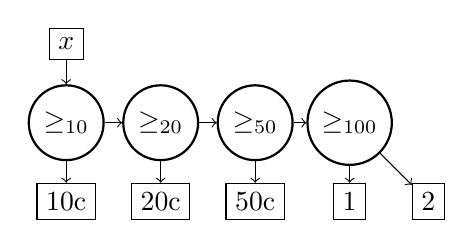
\begin{tikzpicture}
    \tikzstyle{node}=[circle,thick,draw=black,minimum size=4mm]
    \tikzstyle{arg}=[rectangle,thin,draw=black,minimum size=4mm]

    \begin{scope}
      \node[arg](in){$x$};

      \node[node,below of=in](s10){$\ge_{10}$};

      \node[node,right of=s10,xshift=2mm](s20){$\ge_{20}$};
      \node[arg,below of=s10](o10){$10$c};

      \node[node,right of=s20,xshift=2mm](s50){$\ge_{50}$};
      \node[arg,below of=s20](o20){$20$c};

      \node[node,right of=s50,xshift=2mm](s1){$\ge_{100}$};
      \node[arg,below of=s50](o50){$50$c};

      \node[arg,below of=s1](o1){$1$\euro};
      \node[arg,right of=o1](o2){$2$\euro};

      \path[->]
      (in) edge (s10)
      (s10) edge (o10)
      (s10) edge (s20)
      (s20) edge (o20)
      (s20) edge (s50)
      (s50) edge (o50)
      (s50) edge (s1)
      (s1) edge (o1)
      (s1) edge (o2);
    \end{scope}
  \end{tikzpicture}  
  
  \caption{The coffee machine circuit. On input $r\in R$, the operator
    $\ge_x:R\ra R\uplus R$ gives $r$ on its first output if $r\ge x$, on its
    second output otherwise. The circuit is an euro coin separator.}
  \label{fig:coffee}
\end{figure}

In some cases, howevever, evaluation and coevaluation coincide. The
following lemma shows one important case when this happens.

\begin{lemma}
  \label{th:coeval}
  Let $C$ be a circuit over $(R,\Tbasis)$. In the category $\RMod{R}$
  $\eval_C\simeq\lave_C$.
\end{lemma}
\begin{proof}
  For finite dimensional modules, the product and the direct sum are
  the same object. More formally, when working in $\RMod{R}$ there is
  a natural isomorphism $\prod^n R\simeq\coprod^n R$ for any $n$ (this
  is true for any additive category, see \cite[VIII.2]{McLane}). Thus
  $\Tbasis$ is both a basis and a cobasis, up to isomorphism, and both
  evaluation and coevaluation of circuits over it are meaningful.

  The rest of the proof is just induction on the size of the
  circuit. First, it is obvious that for elementary circuits with an
  unique evaluation node $v$ we have $\eval_C \simeq \beta(v) \simeq
  \lave_C$. Then it suffices to show that the property is maintained
  upon composition of circuits.
\end{proof}

The equivalence of evaluations and coevalutions suggests that there is
some unexploited symmetry in circuits over $\Tbasis$. The next
section explores it.


\subsection{The transposition theorem}
\label{sec:tellegen}

Since we are in a non-commutative setting, we have to precisely define
what we mean by ``transposition''. We start by recalling some well
known facts.


The transposition theorem says that from a circuit that computes the
matrix-vector product $x\mapsto \trans{x}M$ for a fixed matrix $M$, one can
deduce another circuit that computes $y\mapsto My$. We now
give such construction.

\begin{definition}[Dual circuit]
  \label{def:dual}
  Let $C=(V,E)$ be a circuit over $(R,\Tbasis)$, the dual circuit of
  $C$, noted $\dual{C}$, is the arithmetic circuit $\dual{C} = (V',
  E)$ over $(R^{\op},\Tbasis)$ where for any node $v=(I,O,f)$ in $V$
  there is a node $\dual{v}=(O,I,f')$ in $V'$ where
  \begin{equation}
    \label{eq:dual-circuit}
    f' = \begin{cases}
      \rmul{a} & \text{if $f = \rmul{a^\op}$}\\
      + & \text{if $f = \hub$}\\
      \hub & \text{if $f = +$}\\
      \omega & \text{if $f = 0$}\\
      0 & \text{if $f = \omega$}
    \end{cases}
  \end{equation}
  The ordering of $V'$ is the same as the one of $V$.
\end{definition}

In particular, this makes $(V',E)$ the reverse graph of $(V,E)$ in a
graph-theoretic sense. Figure \ref{fig:circuit} shows two circuits
that are each other's dual.

\begin{theorem}[Transposition theorem, Fiduccia '72]
  \label{th:tellegen}
  Let $C$ be a circuit over $(R,\Tbasis)$ that computes a module
  homomorphism $f$, then $\dual{C}$ computes the dual homomorphism
  $\dual{f}$.
\end{theorem}
\begin{proof}
  We apply the functor $\dual{()}$ to the construction of $\eval_C$ as
  defined in \ref{def:eval}. It is routine to verify that
  \begin{itemize}
  \item canonical projections in $\RMod{R}$ are taken to canonical
    injections in $\RMod{R^\op}$;
  \item products are taken to coproducts, in particular
    $\dual{\left(\prod^n R\right)} \simeq \coprod^nR^\op$ and the isomorphism is canonical;
  \item any morphism $t\in\Tbasis$ is taken it to its dual $\dual{t}$
    in $\Tbasis^\op$, the same correspondences as in equation
    \eqref{eq:dual-circuit} hold.
  \end{itemize}
  Furthermore, since $\dual{()}$ is contravariant, all the arrows are
  reversed. By comparing this with definitions \ref{def:coeval} and
  \ref{def:dual}, we clearly see that up to a natural isomorphism
  $\dual{\eval_C}\simeq\lave_{\dual{C}}$.

  The claim follows from lemma \ref{th:coeval}.
\end{proof}

\begin{corollary}
  A linear function $f:R^n\ra R^m$ and its dual can be computed by
  arithmetic circuits of same sizes and depths. In particular if $C$
  computes $f$ and $\dual{C}$ computes $\dual{f}$,
  \begin{gather*}
    \size_{\{+\}}(C) = \size_{\{\hub\}}(\dual{C}), \qquad  
    \size_{\{\hub\}}(C) = \size_{\{+\}}(\dual{C}), \\
    \size_{\{\rmul{a}\}}(C) = \size_{\{\rmul{a}\}}(\dual{C})\quad\text{for any $a\in R$},\\
    \size_{\{0\}}(C) = \size_{\{\omega\}}(\dual{C}), \qquad 
    \size_{\{\omega\}}(C) = \size_{\{0\}}(\dual{C}).
  \end{gather*}
\end{corollary}

In the commutative world, if $M$ is the matrix associated to the
homomorphism $f$, $\trans{M}$ is the matrix associated to $\dual{f}$
(up to isomorphism), but when $R$ is not commutative
$\trans{(AB)}\ne\trans{B}\trans{A}$ and this correspondence fails. We
can nevertheless define another transformation on circuits that acts
in a way similar to transposition in some special cases.

\begin{definition}[Opposite circuit]
  Let $C=(V,E)$ be a circuit over $(R,\Tbasis)$, the \emph{opposite
    circuit} of $C$, noted $C^\op$, is the arithmetic circuit over
  $(R^{\op},\Tbasis)$ where any $\beta(v)=\rmul{a}$ has been changed to $\rmul{a^\op}$.
\end{definition}

Now the opposite of a circuit certainly computes some $R^\op$-module
homomorphism, but there is no unique relationship between $\eval_C$
and $\eval_{C^\op}$ due to the lack of commutativity. A special case
of interest is stated in the next corollary.

\begin{definition}[Bilinear chain]
  Let $R$ be non-commutative and let $S\subset R$ be a subring of its
  center. A circuit $C$ over $(R,\Tbasis)$ such that no directed path
  in $C$ contains two nodes $v\ne v'$ with $\beta(v)=\rmul{a}$ and
  $\beta(v')=\rmul{a'}$ where $a,a'\not\in S$ is called an
  $S$-\emph{bilinear chain}.
\end{definition}

\begin{corollary}
  Let $C$ be a bilinear chain and let $\eval_C(x)=\trans{x}M$ for some
  matrix $M$, then $\eval_{C^\op}(x)=\trans{M}x$.
\end{corollary}
\begin{proof}
  Let $x_1,\ldots,x_n$ be the inputs of $C$ and $y_1,\ldots,y_m$ its
  outputs and let $M$ be the $n\times m$ matrix associated to
  $\eval_C$. Each path connecting $x_i$ to $y_j$ contributes linearly
  to the entry $(M)_{i,j}$; more precisely, let $p$ be a path from
  $x_i$ to $y_j$ and let $\rmul{a_1},\ldots,\rmul{a_h}$ be the
  multiplication nodes appearing (in that order) on it, we associate
  to $p$ the element $C_p=a_1\cdots a_h\in R$, then
  \begin{equation}
    (M)_{i,j}=\sum_{p\in\mathcal{P}(x_i,x_j)}C_p
  \end{equation}
  where $p$ ranges over the paths from $x_i$ to $x_j$. Obviously, to
  any path in $C$ corresponds an unique path in $C^\op$, by nothing
  them with the same letter $p$ we have
  \begin{equation}
    C_p^\op=a_1^\op\cdots a_n^\op=(a_n\cdots a_1)^\op=(C_p)^\op
    \text{ ,}
  \end{equation}
  where the last equality comes from the fact that all the $a_i$
  except at most one are in the center of $R$. We conclude that if
  $M'$ is the matrix associated to $C^\op$ then
  \begin{equation}
    (M')_{i,j}=\sum_{p\in\mathcal{P}(x_i,x_j)}C_p^\op=(M)_{i,j}^\op
    \text{ ;}
  \end{equation}
  and thus $\trans{x}M'=\trans{\left(\trans{M}x\right)}$.
\end{proof}



\subsection{Uniformity}
\label{sec:uniformity}

A circuit is limited to compute one specific function with inputs and
outputs of fixed size (in term of elements of $R$). However complexity
theory is interested in algorithms that compute on inputs of variable
size. This will lead us to study families of circuits.

\begin{definition}[Circuit family]
  Let $R$ be a ring, $\mathcal{B}$ a basis over $R$ and $\pspace$ a
  set. A \emph{circuit family} over $(R,\mathcal{B},\pspace)$ is a
  family of circuits over $(R,\mathcal{B})$ indexed by $\pspace$.
  $\pspace$ is called the \emph{parameter space} of the family.
\end{definition}

Algebraic complexity textbooks usually take $\pspace=\N$ and force
$C_n$ to have $n$ inputs. Our construction is more general and its
interest will be clear in the next sections.

\begin{definition}[Size and depth functions]
  Let $\mathcal{C} = (C_j)_{j\in\pspace}$ be a circuit family, we
  define the size and depth function as
  \begin{align*}
    \size^{\mathcal{C}}:\pspace&\ra\N  & \depth^{\mathcal{C}}:\pspace&\ra\N\\
                   j&\mapsto\size(C_j) &    j&\mapsto\depth(C_j)
  \end{align*}
  respectively.

  As in definition \ref{def:size}, for $X\subset\mathcal{B}$ we also
  define
  \begin{align*}
    \size^{\mathcal{C}}_X:\pspace&\ra\N\\
                     j&\mapsto\size_X(C_j)
                     \text{ .}
  \end{align*}
\end{definition}

Circuit families are interesting in theory and theorem
\ref{th:tellegen} easily generalizes to them. However this model of
computation is strictly more powerful than the BSS one (see \cite[Obs.
2.3]{Vollmer}). It is sometimes desirable to restrict oneself to a
more constrained model.

\begin{definition}[Uniform circuit family]
  Let $\mathcal{C} = (C_j)_{j\in\pspace}$ be a circuit family. Fix a
  binary representation of arithmetic circuits over $(R,\mathcal{B})$
  and a binary representation of $\pspace$.

  $\mathcal{C}$ is said to be uniform if there is a multi-band Turing
  machine $\mathcal{M}$ that on input $x$ writes the binary
  representation of $C_x$ on its output tape if $x$ is the binary
  representation of an element of $\pspace$, or an error token otherwise.

  The complexity of $\mathcal{M}$ is called the \emph{uniform
    complexity} of $\mathcal{C}$.
\end{definition}

We are mainly interested in uniform circuit families since they are
equivalent to computable functions, theorem \ref{th:tellegen} easily
generalizes to them. We won't study uniform circuit families more in
depth. Instead, we directly work on computer programs that implicitly
represent circuit families, and automatically deduce the transposed
family without actually using the circuit model. More details on
uniform circuit families can be found in \cite{Vollmer}.



% Local Variables:
% mode:flyspell
% ispell-local-dictionary:"american"
% mode:TeX-PDF
% mode:reftex
% TeX-master: "../these"
% End:
%

\section{Multilinearity}
\label{sec:multi}

In this section we develop an extension of the transposition theorem
to the multilinear case.  The subject has already been treated by
Hopcroft and Musinski \cite{hopcroft+musinski73} and Fiduccia
\cite{fiduccia:phd}, this section is a mild generalization of their
methods.

\subsection{Multilinear circuits}
\label{sec:multilinear-circuits}
We shall consider \index{multilinear~circuit}\emph{multilinear
  circuits}, i.e.\ circuits that, besides the operators
of~\ref{eq:tbasis}, also contain binary multiplication nodes. The
definitions of the previous section must be adapted to deal with
operators that are not module morphisms, but this generalization is
straightforward (see also Appendix~\ref{cha:basic-categ-theory} for a
clean way of defining arithmetic circuits that supports both linear
and arbitrary circuits).

Multilinear circuits are constructed using the
\index{standard~multilinear~basis}\emph{standard multilinear basis}
$\Sbasis$
\begin{equation}
  \label{eq:sbasis}
  \tag{$\Sbasis$}
  \begin{aligned}
    + : R\times R &\ra R\text{,}    & * : R\times R &\ra R\text{,} &  \hub : R &\ra R\times R\text{,}\\
        a, b &\mapsto a+b\text{,}   &     a, b &\mapsto ab\text{,} &         a &\mapsto a,a\text{,}\\ \\
    \eta_a : \{\bom\} &\ra R\text{,}     &&& \omega : R &\ra \{\bom\}\text{,} \\
          \bom &\mapsto a\text{,} &&&          a &\mapsto \bom\text{.}
  \end{aligned}
\end{equation}


We are going to define a transformation process that transforms a
circuit over $(R,\Sbasis)$ in a (uniform) circuit family over
$(R,\Tbasis)$; the idea is to make any bilinear multiplication node
linear by \emph{fixing} one of its inputs (see
Figure~\ref{fig:linearization}). We call this process
\emph{linearization}, a special case of it has been used in
\cite{gashkov+gashkov05,sergeev08} to transpose circuits that compute
differentials.

\begin{definition}[Zero edge, null edge]
  Let $C$ be a circuit over $(R,\Sbasis)$, a \emph{zero edge} is any
  edge $e$ in $C$ such that one of the following conditions holds:
  \begin{itemize}
  \item $e$ stems from a node $v$ with $\beta(v)=\eta_0$, such an edge
    is also called a \emph{normal} zero edge;
  \item $e$ stems from a node $v$ with $\beta(v)=+$ and whose incident
    edges are both zero;
  \item $e$ stems from a node $v$ with $\beta(v)=*$ and such that at
    least one of the incident edges of $v$ is zero;
  \item $e$ stems from a node $v$ with $\beta(v)=\hub$ and whose input
    edge is zero.
  \end{itemize}
  A \emph{null edge} is any edge $e$ such that one of the following
  conditions holds:
  \begin{itemize}
  \item $e$ is incident to a node $v$ with $\beta(v)=\omega$, such an
    edge is also called a \emph{normal} null edge;
  \item $e$ is incident to a node $v$ with $\beta(v)=\hub$ and whose
    stemming edges are both null;
  \item $e$ is incident to a node $v$ with $\beta(v)\in\{+,*\}$ such
    that its stemming edge is null.
  \end{itemize}
  An output node whose incident edge is zero is called a \emph{zero
    output}, an input node whose stemming edge is null is called a
  \emph{null input}.  A \emph{normal} circuit is a circuit whose zero
  and null edges are all normal.
\end{definition}

Notice that the evaluation of a zero edge or output is the zero
function, the converse is not true.  There is an obvious normalization
technique that takes a generic circuit and transforms it in a normal
circuit having the same evaluation; clearly, the normalization does
not increase the size and the depth of the circuit (it generally
increases $\size_{\{\eta_0,\omega\}}$, though). When necessary, we
will restrict ourselves to normal circuits.

\begin{definition}[Linearization]
  \label{def:linearization}
  \index{linearization}
  Let $C=(V,E)$ be a circuit over $(R, \Sbasis)$. Let $0=\{v\in
  V|\beta(v)=\eta_0\}$, a linearization of $C$ is a subset
  $\ell\subset\inp(C)\cup 0$ such that:
  \begin{itemize}
  \item for every $v\in V$ with $\beta(v)=+$ either none of its
    incident edges is reachable from $\ell$, or both are;
  \item for every $v\in V$ with $\beta(v)=*$ at most one of the edges
    incident to $v$ is reachable from $\ell$; if $R$ is
    non-commutative, such edge is always the right (left) edge and the
    linearization is called a
    \index{linearization!left}\index{linearization!right}\emph{left
      (right) linearization}.
  \end{itemize}
  If $\ell=\emptyset$, the linearization is called
  \index{linearization!trivial}\emph{trivial}.

  The elements of $\ell\cap\inp(C)$ and $s = \inp(C) - \ell$ are
  respectively called the \index{linear~input}\emph{linear} and
  \index{scalar~input}\emph{scalar} inputs. An edge reachable from
  $\ell$ is called \index{linear~edge}\emph{linear},
  \index{scalar~edge}\emph{scalar} otherwise.
\end{definition}


\begin{definition}[Linearized circuit, scalar part]
  Let $C=(V,E,\le,\le_i,\le_o)$ be a normal circuit over $(R,\Sbasis)$
  and let $\ell$ be a left (resp. right) linearization; without loss
  of generality, we suppose that all the scalar inputs precede the
  linear inputs in the order $\le_i$ (one can always permute inputs).
  
  Let $n$ be the number of scalars for the linearization $\ell$ and
  let $x_1,\ldots,x_n$ be distinct indeterminates over $R$. The
  \index{linearized~circuit}\emph{linearized circuit}
  \begin{equation*}
    C_\ell=(V_\ell,E_\ell,\le_\ell,\le_{i,\ell},\le_{o,\ell})
  \end{equation*}
  is the circuit over $(R[x_1,\ldots,x_n], \Tbasis)$
  (resp. $(R^\op[x_1,\ldots,x_n],\dual{\Tbasis})$) obtained from $C$
  as follows:
  \begin{itemize}
  \item $E_\ell$ is the subset of $E$ containing the linear edges,
  \item $V_\ell$ are the nodes of $V$ adjacent to $E_\ell$, where
    $\beta(v)$ has incurred the following substitutions:
    \begin{itemize}
    \item $\eta_0$ becomes $0$; $+, \hub, \omega$ are preserved;
    \item if $\beta(v)=*$, let $e$ be the only non-linear edge
      incident to $v$ and let
      $a=\eval_e(x_1,\ldots,x_n,\bullet,\ldots,\bullet)$, then $*$
      becomes $\rmul{a}$;
    \item The orders $\le_\ell,\le_{i,\ell},\le_{o,\ell}$ are the
      restriction to $V$ of the original ones.
    \end{itemize}
  \end{itemize}

  The sets $V-V_\ell$ and $E-E_\ell$ are called the \emph{scalar part}
  of $C$.
\end{definition}

Observe that non-linear edges do not depend on linear inputs, thus the
substitution for $*$ is well defined. The trivial linearization gives
the trivial linear circuit with no nodes, hence, its evaluation is the
trivial map $0\ra0$. Figure \ref{fig:linearization} shows an example
of linearized circuit (in the case $R$ is commutative), we gray out
the scalar part of the circuit.

\begin{figure}[!ht]
  \centering
  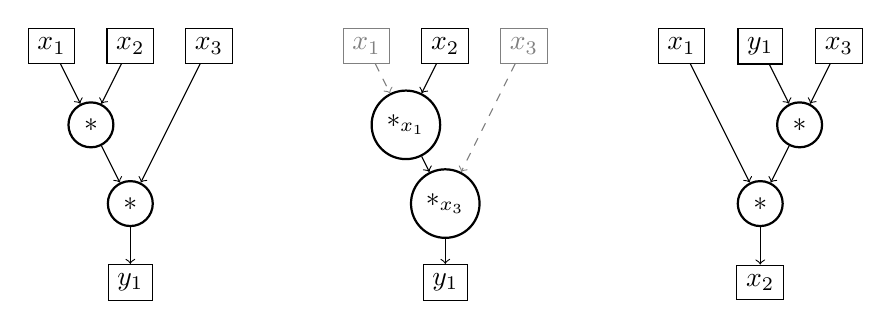
\begin{tikzpicture}
    \tikzstyle{node}=[circle,thick,draw=black,minimum size=4mm]
    \tikzstyle{arg}=[rectangle,thin,draw=black,minimum size=4mm]
    \tikzstyle{nodeg}=[circle,thick,draw=gray,minimum size=4mm]
    \tikzstyle{argg}=[rectangle,thin,draw=gray,minimum size=4mm]
    
    \begin{scope}
      \node[arg](in1){$x_1$};
      \node[arg,right of=in1](in2){$x_2$};
      \node[arg,right of=in2](in3){$x_3$};
      \node[node,below of=in1,xshift=5mm](times1){$*$};
      \node[node,below of=times1,xshift=5mm](times2){$*$};
      \node[arg,below of=times2](out){$y_1$};

      \path[->]
      (in1) edge (times1)
      (in2) edge (times1)
      (times1) edge (times2)
      (in3) edge (times2)
      (times2) edge (out);
    \end{scope}

    \begin{scope}[xshift=4cm]
      \node[argg](in1){\color{gray}{$x_1$}};
      \node[arg,right of=in1](in2){$x_2$};
      \node[argg,right of=in2](in3){\color{gray}{$x_3$}};
      \node[node,below of=in1,xshift=5mm](times1){$\rmul{x_1}$};
      \node[node,below of=times1,xshift=5mm](times2){$\rmul{x_3}$};
      \node[arg,below of=times2](out){$y_1$};

      \path[->]
      (in2) edge (times1)
      (times1) edge (times2)
      (times2) edge (out);
      
      \path[->,draw=gray,dashed]
      (in1) edge (times1)
      (in3) edge (times2);
    \end{scope}

    \begin{scope}[xshift=8cm]
      \node[arg](in1){$x_1$};
      \node[arg,right of=in1](in2){$\dual{y_1}$};
      \node[arg,right of=in2](in3){$x_3$};
      \node[node,below of=in3,xshift=-5mm](times1){$*$};
      \node[node,below of=times1,xshift=-5mm](times2){$*$};
      \node[arg,below of=times2](out){$\dual{x_2}$};

      \path[->]
      (in2) edge (times1)
      (times1) edge (times2)
      (times2) edge (out)
      (in1) edge (times2)
      (in3) edge (times1);
    \end{scope}
  \end{tikzpicture}
  \caption{A circuit over a commutative ring, its linearization for
    $\ell=\{x_2\}$ (scalar edges are grayed out) and its
    $\ell$-dual.}
  \label{fig:linearization}
\end{figure}

Any linearized circuit obviously defines an uniform circuit family
over $(R,\Tbasis)$ (resp. $(R^\op,\dual{\Tbasis})$), thus we can apply
the transposition theorem to the family. But there's more: from a
linearized circuit we can deduce a new circuit over $(R,\Sbasis)$ that
computes the same function as the transposed family.

\begin{definition}[$\ell$-dual]
  \label{def:ell-dual}\index{arithmetic~circuit!l-dual@$\ell$-dual}
  Let $C$ be a normalized circuit over $(R,\Sbasis)$ and let $\ell$ be
  a linearization.  The $\ell$-dual of $C$ is the circuit over
  $(R,\Sbasis)$ obtained by dualizing the linearized circuit $C_\ell$,
  then connecting back the edges of the scalar part to the
  corresponding nodes in $C_\ell$: in doing this nodes with
  $\beta(v)=\rmul{a}$ are changed back to $\beta(v)=*$. The order on
  the nodes of the $\ell$-dual is arbitrary.
\end{definition}

By abuse of notation, the $\ell$-dual will also be noted
$\dual{C_\ell}$. Figure \ref{fig:linearization} shows an example of
$\ell$-dual; notice that $\dual{C_\ell}$ is only defined up to
reordering of the nodes, we will adopt the convention of preserving
the ordering of the linearized circuit, while we take the freedom to
permute the scalar part as it will be more convenient.

\begin{proposition}
  The size of the $\ell$-dual is the same as that of $C$, more
  precisely
  \begin{align*}
    \size_{\{+,\hub\}}(C) &= \size_{\{+,\hub\}}(\dual{C_\ell}), 
    &\size_{\{*\}}(C) &= \size_{\{*\}}(\dual{C_\ell}),\\
    \size_{\{\eta_0,\omega\}}(C) &= \size_{\{\eta_0,\omega\}}(\dual{C_\ell}), 
    &\size_{\{\eta_a|a\ne0\}}(C) &= \size_{\{\eta_a|a\ne0\}}(\dual{C_\ell}).
  \end{align*}
  Its depth is at most twice that of $C$.
\end{proposition}


\subsection{Bilinear chains}
\label{sec:bilinear-chains}

The case of bilinear circuits has received particular interest because
it permits to give lower bounds on the complexity of matrix
multiplication~\cite{fiduccia:phd}. In this section we just point out
how the results of Hopcroft and Musinski~\cite{hopcroft+musinski73}
and Fiduccia~\cite{fiduccia:phd} reduce to ours.

\begin{definition}[Linear chain]
  Let $R$ be non-commutative and let $S\subset R$ be a subring of its
  center. A circuit $C$ over $(R,\Tbasis)$ such that no directed path
  in $C$ contains two nodes $v\ne v'$ with $\beta(v)=\rmul{a}$ and
  $\beta(v')=\rmul{a'}$ where $a,a'\not\in S$ is called an
  \index{linear~chain}\emph{$S$-linear chain}.
\end{definition}

We have seen in Remark~\ref{rk:tellegen} that in the non commutative
case the transposition principle does not \emph{transpose
  matrices}. It is however possible to transpose linear chains.

\begin{definition}[Opposite circuit]
  Let $C=(V,E)$ be a circuit over $(R,\Tbasis)$, the
  \index{arithmetic~circuit!opposite}\emph{opposite circuit} of $C$,
  noted $C^\op$, is the arithmetic circuit over $(R^{\op},\Tbasis)$
  where any $\beta(v)=\rmul{a}$ has been changed to $\rmul{a^\op}$.
\end{definition}

\begin{proposition}
  Let $C$ be a linear chain and let $\eval_C(x)=\trans{x}M$ for some
  matrix $M$, then $\eval_{C^\op}(x)=\trans{M}x$.
\end{proposition}
\begin{proof}
  This is a consequence of the
  \hyperref[th:electrical-network]{electrical network lemma}.  The
  matrix $M$ associated to $\eval_C$ is given by
  \begin{equation}
    \label{eq:243}
    m_{ij} = \pi_j\circ\eval_C\circ\iota_i(1)
    = \sum_{p\in x_i\leadsto y_j}\eval_p(1) =
    \sum_{p\in x_i\leadsto y_j} p_1p_2\cdots p_{n_p}
    \text{,}
  \end{equation}
  where $\rmul{p_1},\ldots,\rmul{p_{n_p}}$ are the scalar
  multiplication nodes on the path $p$.

  Now, by the definition of linear chain, on any path there is at most
  one element not in the center of $R$, thus
  \begin{equation}
    \label{eq:245}
    (p_1p_2\cdots p_{n_p})^\op=p_{1}^\op p_2^\op\cdots p_{n_p}^\op
    \text{,}
  \end{equation}
  and the claim follows.
\end{proof}

Thus, to any linear chain one can associate the four circuits
$C,\dual{C},C^\op,\dual{{C^\op}}$. In~\cite{hopcroft+musinski73,fiduccia:phd},
bilinear chains are considered, i.e.\ bilinear circuits whose only two
non-trivial linearizations are linear chains. The opposite circuit of
a \index{bilinear~chain}bilinear chain is defined by swapping every
multiplication node. Thus, if $C$ is a bilinear chain and
$\ell_1,\ell_2$ its linearizations, one obtains the six circuits
\[C,C^\op,\dual{C_{\ell_1}},\dual{{C_{\ell_1}^\op}},\dual{C_{\ell_2}},\dual{{C_{\ell_2}^\op}}\text{.}\]

Finally, the complexity bounds of~\cite{hopcroft+musinski73}, are
obtained by considering the sets $D=\{\rmul{a}|a\in S\}$ and
$M=\{\rmul{a}|a\not\in S\}$ and realizing that both $\size_D$ and
$\size_M$ are preserved taking the $\ell$-dual and/or the opposite.



% Local Variables:
% mode:flyspell
% ispell-local-dictionary:"american"
% mode:TeX-PDF
% mode:reftex
% TeX-master: "../these"
% End:
%

\section{From circuits to function-level programming}
\label{sec:fp}
\lstset{language=haskell}

In Section \ref{sec:circuits} we saw that the transposition theorem
holds for uniform circuit families.  Informally, an uniform circuit
family can be simulated in a BSS-like model \cite{BSS} such as a
Turing machine with an additional input/output tape where each cell
contains an element of $R$. Then the transposition theorem can be
extended to this context and it is easy to prove that some fundamental
measures such as space and time complexity are preserved by it. This
kind of approach has been used in \cite{BoLeSc03}.

We won't go further in defining a model and proving a transposition
theorem as this is just matter of posing the right definitions and
deriving the (boring) consequences. Here, instead, we are interested
in the real world scenario of transposing a computer program written
in a general purpose programming language. This section studies how an
uniform circuit family can be efficiently simulated in the Haskell
programming language and how its transposition can automatically be
obtained. Nevertheless, this approach has some limitations that we
will address in the next sections.

As we already pointed out in Section \ref{sec:circuits}, evaluation
(and co-evaluation) of arithmetic circuits can be formally defined by
means of a category with finite products (and coproducts). Arithmetic
circuits over $\Tbasis$, in particular, are defined by means of an
\emph{additive category}, that is a category such that $\hom$ sets are
abelian groups, it has \emph{zero morphisms} and it has all finite
\emph{biproducts}.

It can be proven \cite[VIII.2]{McLane} that in an additive category
finite products and coproducts are naturally isomorphic to biproducts.
This is the key argument for the proof of our lemma \ref{th:coeval}
and ultimately leads to the transposition theorem in the special case
of $\RMod{R}$.

Modern functional languages too are constructed around the concept of
category: roughly, the types of the language are viewed as objects and
programs as arrows. In this setting, categories are required to be
\emph{Cartesian closed}. This allows to perform \emph{partial
  evaluation} of a function, an operation known as
\emph{currying}. Examples of Cartesian closed categories are
$\mathsf{Set}$ and $\mathsf{Hask}$ --the category of Haskell types--.

Cartesian closed categories cannot be additive, thus it may seem that
our attempts to natively express circuits in functional languages are
doomed. However the Haskell type system is powerful enough to
represent some categories inside it, in particular subcategories of
$\mathsf{Hask}$. It provides a \emph{type class} \lstinline+Category+,
that we reproduce here --following \cite{Yor09}, we use an infix
operator \lstinline+(~>)+ instead of a prefix one as in the standard
Haskell library--.

\begin{lstlisting}
  class Category (~>) => where
    id :: (a ~> a)
    (.) :: (b ~> c) -> (a ~> b) -> (a ~> c)
\end{lstlisting}

In order to behave as a category, an instance of this class shall form
a monoid for the operation \lstinline+(.)+, with \lstinline+id+ being
the identity element. Now this class can be extended to model additive
categories: we first define a class that mimics \emph{Ab-categories},
or \emph{preadditive} categories, that is categories whose $\hom$ sets
are abelian groups.

\begin{lstlisting}
  class Category (~>) => AbCategory (~>) where
    zeroArrow :: (a ~> b)
    (<+>) :: (a ~> b) -> (a ~> b) -> (a ~> b)
\end{lstlisting}
To behave as an Ab-category, an instance shall form an abelian group
for the operation \lstinline|<+>|, with \lstinline+zero+ being the
identity element; it shall also obey a \emph{bilinear law}:
\begin{lstlisting}
  (f <+> g).(h <+> i) = f.h <+> f.i <+> g.h <+> g.i
\end{lstlisting}

Now we give one possible definition of a class that mimics additive
categories.
\begin{lstlisting}
  class AbCategory (~>) => AdditiveCategory (~>) where
    (&&&) :: (a ~> b) -> (a ~> c) -> (a ~> (b, c))
    (|||) :: (a ~> c) -> (b ~> c) -> ((a, b) ~> c)

  first f = f <**> zeroArrow
  second f = zeroArrow <**> f
  left f = f <++> zeroArrow
  right f = zeroArrow <++> f
  f *** g = (first f) ||| (second g)
\end{lstlisting}
For an instance to behave as an additive category it shall satisfy
\begin{lstlisting}
  id *** id = id
  zeroArrow &&& zeroArrow = zeroArrow ||| zeroArrow = zeroArrow
  (f &&& g) <+> (f' &&& g') = (f <+> f') &&& (g <+> g')
  (f ||| g) <+> (f' ||| g') = (f <+> f') ||| (g <+> g')
  (f ||| g) &&& (f' ||| g') = (f &&& f') ||| (g &&& g')
  (f ||| g)  .  (f' &&& g') = f.f' <+> g.g'
\end{lstlisting}

Haskell programmers may have recognized a familiar pattern:
\emph{arrows}. Arrows were introduced in \cite{Hug00} as a
generalization of \emph{monads}, they have been successfully applied
to many different settings such as, for example, solving ordinary
differential equations \cite{LH10}. They are usually understood as
circuits \cite{Pat01}: the standard library class \lstinline+Arrow+ is
roughly equivalent to evaluation of an arithmetic circuit in
$\mathsf{Hask}$ (or $\mathsf{Set}$), while \lstinline+ArrowChoice+ is
roughly equivalent to co-evaluation.

Our \lstinline+AdditiveCategory+ shares similarities with the standard
classes \lstinline+Arrow+, \lstinline+ArrowChoice+,
\lstinline+ArrowZero+ and \lstinline+ArrowPlus+. In particular, it is
equivalent to evaluation of an arithmetic circuit in an additive
category and, by lemma \ref{th:coeval}, to co-evaluation.

An arrow expression is an expression formed uniquely from elementary
arrows and the combinators of \lstinline+AdditiveCategory+. Given an
arrow expression, it is trivial to form its dual: one substitutes
\lstinline|first| with \lstinline|left|, \lstinline|second| with
\lstinline|right|, \lstinline|&&&| with \lstinline&|||& and changes
any \lstinline|f.g| into \lstinline|g.f|. This corresponds to forming
the dual circuit as in definition \ref{def:dual}, thus if
\lstinline+AdditiveCategory+ is instantiated with arrows that
correspond to the elements of the basis\footnote{It is actually enough
  to create the elementary arrows that correspond to $*_a$ for any
  $a\in R$. The combinators \lstinline+&&&+ and \lstinline+|||+
  already imply $+$ and $\hub$.} $\Tbasis$, one obtains the transposed
circuit as in theorem \ref{th:tellegen}. Also notice that Haskell
defines a \lstinline+do+-notation \cite{Pat01} to write down arrow
expressions more conveniently. Dualizing this notation boils down to
applying the transposition algorithm given in Section \ref{todo}.

By writing Haskell functions that return arrows, or, more generally,
functions that have arbitrary types involving arrows, one can express
circuit families and apply the transposition theorem to them by
dualizing each arrow expression appearing in the computation. Figure
\ref{fig:karahask} shows an example of Karatsuba multiplication
written using this technique.

\begin{figure}
  \centering
  
  \caption{The left-linear Karatsuba algorithm.}
  \label{fig:karahask}
\end{figure}


One limitation to this approach is that it cannot be implemented
inside Haskell. As we have defined them, arrows do not remember their
history: the arrow \lstinline+f.g+ is a new arrow that knows nothing
about the pieces that compose it, thus no Haskell function can
transform it in \lstinline+g.f+. There are three solutions to this:
\begin{enumerate}
\item Define \emph{biarrows} instead of arrows \cite{ASWEP05}. This
  way the dual is computed as a side effect of the computation of the
  arrow. The main advantage of this approach is that it is easy to
  implement, its main disadvantage is that it is not compatible with
  the \lstinline+do+ notation, as observed in \cite{ASWEP05}. Another
  minor disadvantage is that the dualization is not transparent as it
  does not happen at the level of the arrow expression, but inside its
  computation.
\item Write a precompiler for Haskell that dualizes arrow
  expressions. The great advantage of this approach is that it permits
  to treat \lstinline+do+-expressions.
\item Implement arrows at the type-level, instead of the function
  level, by defining a type that describes circuits. However this
  approach is not realistic because of its poor efficiency.
\end{enumerate}

A second, fundamental, limitation is that this approach requires the
user to explicitly identify the linear computations by wrapping them
in arrows. This process may be almost as hard as transposing a program
by hand as done by \cite{BoLeSc03} and the resulting code may be
difficult to read (see figure \ref{fig:karahask}). The next Section
studies an alternative approach where the user if freed from the
burden of \emph{linearizing} the program.



% Local Variables:
% mode:flyspell
% ispell-local-dictionary:"american"
% mode:TeX-PDF
% TeX-master: "transAL"
% End:
%

In this chapter we present a joint work with
Schost~\cite{df+schost10}. We study the
\index{automatic~transposition}\emph{automatic transposition} of
generic code (i.e.\ not limited to straight line programs).
Section~\ref{sec:autom-diff} has shown that this has applications in
automatic differentiation, and we will see other applications in the
next chapters.

By looking at a specific subproblem of automatic differentiation, our
goal is to be more efficient and more general. In particular, compared
to the existing implementations of AD tools, we want to:
\begin{itemize}
\item avoid unnecessary space overhead;
\item handle algebraic, rather than just numerical code;
\item handle advanced programming constructs, including recursion and
  algebraic data types;
\item transpose code parameterized by arbitrary algebraic variables.
\end{itemize}

In this chapter we shall abandon the algebraic RAM model we used in
Section~\ref{sec:stra-line-progr} and work on source code
transformation. Implementation details such as knowing what the cost
of copying variables is, shall be ignored: one can assume that a good
compiler will optimize most of these details. Hence, we shall assume
that Theorem~\ref{th:tellegen-R-algeb} really reflects the behavior of
the code we generate.


\section{Inferring linearity}
\label{sec:inference}
\lstset{language=haskell}

By looking at Section~\ref{sec:transp-algor} one sees that often we
want to transpose families of $R$-algebraic algorithms parameterized
by algebraic elements (e.g., we want to transpose the code that for
any $a\in R$ evaluates the map $b\mapsto ab$). This is also necessary
in automatic differentiation, when the code for $\diff_x f$ not only
depends on $\diff x_1,\ldots,\diff x_n$, but also on $x$.

The next section will address the question of how to transpose such
code. This section, instead, asks the question: can a compiler guess
by itself which inputs to a function are parameters, and which are
linear arguments?

The answer is yes. We show how the type system of common statically
typed functional languages can be extended to automatically infer all
the possible \index{linearization}\emph{linearizations} of a computer
program. We first present the non-commutative case, which can be fully
expressed inside the Haskell type system, then we discuss how to
extend to the commutative case.

\paragraph{Linears, scalars}
\label{sec:linears-scalars}
Suppose we have defined some data type \lstinline{R} representing
elements of a ring $R$ together with the usual constants (say
\lstinline{zeroR}, \lstinline{oneR}, etc.), arithmetic operations (say
\lstinline{plus}, \lstinline{times}, etc.), tests and so on. To
simplify, we assume --as usual in algebraic complexity theory-- that
the type \lstinline{R} is isomorphic to $R$, i.e.\ the elements of $R$
can be represented exactly, the operations do not introduce any
rounding error, etc.

For any term involving elements of type \lstinline{R} we would like
the type system to tell us whether its outputs are linear in its
inputs. For example the term
\begin{lstlisting}
  \x y -> plus x y
\end{lstlisting}
has type \lstinline{R -> R -> R}, but we would like the type checker
to also output something like $\ell\ra\ell\ra\ell$ ($\ell$ for
\index{linear~input}\emph{linear}) telling that the term is a
(curryfied) left module homomorphism from $R^2$ to $R$. For
consistency, we want to view constants as mappings from $R^0$ to $R$,
thus for the term \lstinline{zeroR} we want the type checker to
compute something like $0\ra\ell$, that we simply write as $\ell$.

Now, what do we expect about \lstinline{oneR} or \lstinline{times}?
The former is the mapping $\bom\mapsto1$, which is not a module
homomorphism; then, by analogy with
Definition~\ref{def:linearization}, we want the type checker to output
something like $0\ra s$, or simply $s$ ($s$ for
\index{scalar~input}\emph{scalar}). The second can be made into a
linear mapping by \emph{fixing} its second argument (remember that for
the moment we are restricting to left modules) as we did in
Section~\ref{sec:multi}; thus we expect the type checker to output
$\ell\ra s\ra\ell$, meaning that
\begin{lstlisting}
  \x -> times x y
\end{lstlisting}
is a left module homomorphism $R\ra R$ for any \lstinline{y::R}.

Finally consider the following term
\begin{lstlisting}
  z x n = if n <= 0 then zeroR else plus x (z x (n-1))
\end{lstlisting}
as before we expect something like $\ell\ra\N\ra\ell$, meaning that
\begin{lstlisting}
  \x -> z x n
\end{lstlisting}
is a homomorphism $R\ra R$ for any integer \lstinline{n}.

Observe that in order to make a correct inference about a term such as
\begin{lstlisting}
  \x y -> times x (plus y y)
\end{lstlisting}
we must also admit for any of the previous cases the possibility where
everything is a scalar, so that from the hypothesis that
\lstinline{plus} has type $s\ra s\ra s$ we can deduce the correct type
$\ell\ra s\ra\ell$ for the term above. Summarizing, we would like to
have two types \lstinline{L} and \lstinline{S} such that the following
equations hold
\begin{lstlisting}
  plus :: L -> L -> L
  plus :: S -> S -> S
  times :: L -> S -> L
  times :: S -> S -> S
  zeroR :: L
  zeroR :: S
  oneR :: S
\end{lstlisting}

\pdfmcone{Better with newtypes, thanks to Mathieu.}
If we define \lstinline{L} and \lstinline{S} as wrappers around
\lstinline{R}
\begin{lstlisting}
  newtype L = Lin R
  newtype S = Sca R
\end{lstlisting}
then, using Haskell type classes
\cite{Walder+Blott-ad-hoc-polymorphism}, we can conveniently express
all the equations above as
\begin{lstlisting}
  class Ring r where
    zero :: r
    (<+>) :: r -> r -> r
    neg :: r -> r
    (<*>) :: r -> S -> r
\end{lstlisting}
together with the obvious \lstinline{instance} definitions (see the
example in Appendix~\ref{cha:line-infer-karats}). 

\pdfmcone{Better terminology, thanks to Mathieu.}  For our
inference to work, it is important that \lstinline{L} be an abstract
data type with only the above functions in its interface. On the other
hand, any other function acting on \lstinline{R} can be wrapped inside
a function acting on \lstinline{S} as, for example,
\begin{lstlisting}
  one = Sca oneR
  (Sca a) == (Sca b) = a == b
\end{lstlisting}
or, simply, using a \lstinline{deriving} clause in the declaration of
\lstinline{S}
\begin{lstlisting}
  newtype S = Sca R deriving (Eq)
\end{lstlisting}

If we restrict to terms that do not use the type constructor
\lstinline{Lin}, then we can show that the semantic of a term with
type
\begin{lstlisting}
  L->...->L->L
\end{lstlisting}
is a left module homomorphism.  \pdfmcone{More details on the
  simply typed lambda calculus, as suggested by Mathieu.}  The proof
for the full language would be too long, thus we restrict to a simply
typed $\lambda$-calculus with constants. Its terms are defined by the
following grammar
\begin{equation}
  \label{eq:lambda}
  t ::= c \;|\; x \;|\; t_0 t_1 \;|\; \lambda x . t  \text{ ,}
\end{equation}
where $x$ are identifiers and $c$ are constants; its types are
defined by the grammar
\begin{equation}
  \label{eq:77}
  \tau ::= \ell \;|\; s \;|\; \beta \;|\; \tau \ra \tau
  \text{ ,}
\end{equation}
where $\beta$ are the usual base types (integers, booleans, etc.). If
$\Gamma$ is a type environment, by $\Gamma\vdash t::\tau$ we mean that
the term $t$ has type $\tau$ in $\Gamma$.  The semantic of our
calculus is the usual one, based on $\beta\eta$-reduction.

\pdfmcone{Careful about lists and tuples, thanks Mathieu!}  We
suppose all the constants above are defined, plus the usual constants
for the other base types; observe that our grammar forbids type
constructors altogether (including \lstinline{Lin} and
\lstinline{Sca}). In this context we use the type names $\ell$ and $s$
in place of the Haskell types \lstinline{L} and \lstinline{S} defined
above. For simplicity, we shall also assume that lists and tuples are
not part of the types of our language; see the end of this section for
a discussion about them.

\begin{definition}[Flipper]
  \pdfmcone{Defined the flipper and changed the proof of the
    lemma, thanks to Léo.}  Let $\tau$ be the type
  \begin{equation}
    \label{eq:58}
    \tau = \alpha_0\ra\alpha_1\ra\cdots\ra\alpha_n
  \end{equation}
  with $\alpha_n$ not a function type. Let $I\subset[0,\ldots,n-1]$
  such that $\alpha_i\ne\ell$ if and only if $i\in I$, and let
  $m=\card{I}$.  The \emph{flipper} for $\tau$, denoted by $\flip_\tau$,
  is the term
  \begin{equation}
    \label{eq:60}
    \flip_\tau = \lambda t.\lambda x_{i_1}.\ldots.\lambda x_{i_m}.
    \lambda x_{j_1}.\ldots.\lambda x_{j_{n-m}}.tx_0\cdots x_{n-1}
    \text{,}
  \end{equation}
  with $i_1,\ldots,i_m\in I$ and $j_1,\ldots,j_{n-m}\in\bar{I}$.
\end{definition}

\begin{lemma}
  \label{th:lininference}
  Let $\Gamma\vdash t::\tau$ be a term, let $m,n\ge0$, and let
  $\Gamma\vdash \flip_{\tau}t::\sigma$ with
  \begin{equation}
    \label{eq:264}
    \sigma=\alpha_1\ra\alpha_2\ra\cdots\ra\alpha_m\ra\underbrace{\ell\ra\cdots\ra\ell}_{\text{$n$ times}}\ra\beta
    \text{,}    
  \end{equation}
  with $\alpha_i\ne\ell$ and $\beta$ not a function type. Let
  $\Delta_i\vdash s_i::\alpha_i$ for $1\le i\le m$. The semantic of
  \begin{equation}
    \label{eq:270}
    \Gamma,\Delta_1,\ldots,\Delta_m\vdash \flip_\tau ts_1\cdots s_m
  \end{equation}
  is
  \begin{enumerate}
  \item\label{item:1} a constant function if $\beta\ne\ell$,
  \item\label{item:2} a module homomorphism $R^n\ra R$ if $\beta=\ell$,
  \end{enumerate}
  assuming the free variables in $t,s_1,\ldots,s_m$
  satisfy~\ref{item:1} or~\ref{item:2}.
\end{lemma}
\begin{proof}
  We distinguish the following cases.
  \begin{itemize}
  \item $\Gamma\vdash c$. All the constants satisfy
    either~\ref{item:1} or~\ref{item:2}. We just work out $0$ and $+$
    defined above and leave the others to the reader; in both cases
    $\flip_\tau c=c$ up to $\beta\eta$-conversion.
    \begin{itemize}
    \item $\Gamma\vdash0::\ell$ is the map $\bom\mapsto 0$, thus a
      (constant) morphism.
    \item $\Gamma\vdash0::s$ is the map $\bom\mapsto 0$, thus a constant
      (morphism).
    \item $\Gamma\vdash+::\ell\ra\ell\ra\ell$ is the map $a,b\mapsto
      a+b$. A morphism.
    \item $\Gamma\vdash+::s\ra s\ra s$. Take any $a::s$ and $b::s$, then
      $\Gamma\vdash a+b::s$ is a constant.
    \end{itemize}
  \item $\Gamma,x::\alpha\vdash x::\alpha$. The claim follows because
    $x$ is free.
  \item $\Gamma\vdash t_0t_1::\tau$. This is the only real case
    to prove. We distinguish two cases:
    \begin{itemize}
    \item $\Gamma\vdash t_1::\ell$, then, by induction its semantic is
      a morphism $0\ra R$ (because it is $\beta\eta$-equivalent to
      $\flip_\ell t_1$). 

      Let $\Gamma\vdash \flip_\tau t_0t_1::\sigma$, with $\sigma$ as in
      Eq.~\eqref{eq:264}, and let $\Delta_i\vdash s_i$ for $1\le i\le
      m$ be as in the hypothesis.  Let $\Gamma\vdash t_0::\tau_0$ and
      $\Gamma\vdash\flip_{\tau_0}t_0::\sigma_0$, then by induction
      \begin{equation}
        \label{eq:271}
        \Gamma,\Delta_1,\ldots,\Delta_m\vdash t_0'\eqdef\flip_{\tau_0}t_0s_1,\ldots,s_m
      \end{equation}
      is either a morphism $R^{n+1}\ra R$ or a constant function. In
      the first case $t_0't_1$ is a morphism $R^{n'}\ra R$, in the second
      case it is a constant function; in both cases
      \begin{equation}
        \label{eq:74}
        \flip_\tau(t_0t_1)s_1\cdots s_m\xleftrightarrow{\beta\eta}t_0't_1        
      \end{equation}
      and the claim follows.
    \item $\Gamma\vdash t_1::\alpha$ with $\alpha\ne\ell$. Then the
      claim follows directly by induction on $t_0$ and
      $\beta\eta$-conversion, by choosing $s_1=t_1$.
    \end{itemize}
  \item $\Gamma\vdash \lambda x.t::\alpha_1\ra\alpha_2$. By induction
    $\Gamma,x::\alpha_1\vdash t::\alpha_2$ satisfies~\ref{item:1}
    or~\ref{item:2} (assuming $x$ does). We distinguish two cases
    \begin{itemize}
    \item $\alpha_1\ne\ell$, then
      \begin{equation}
        \label{eq:73}
        \lambda x.\flip_{\alpha_2}t\xleftrightarrow{\beta\eta}\flip_{\alpha_1\ra\alpha_2}(\lambda x.t)
        \text{;}
      \end{equation}
    \item $\alpha_1=\ell$, then
      \begin{equation}
        \label{eq:76}
        \lambda x.\flip_{\alpha_2}ts_1\cdots s_m\xleftrightarrow{\beta\eta}
        \flip_{\alpha_1\ra\alpha_2}(\lambda x.t)s_1\cdots s_m
        \text{.}
      \end{equation}
    \end{itemize}
    In both cases, $\lambda x.t$ satisfies~\ref{item:1}
    or~\ref{item:2} accordingly.
  \end{itemize}
\end{proof}

\begin{proposition}
  Let $t:\tau$ be a closed term, let $n\ge0$ and let
  \begin{equation}
    \tau=\underbrace{\ell\ra\cdots\ra\ell}_{\text{$n$ times}}\ra\beta
    \text{,}    
  \end{equation}
  with $\beta$ not a function type. Then, the semantic of $t$ is
  \begin{enumerate}
  \item a constant function if $\beta\ne\ell$,
  \item a module homomorphism $R^n\ra R$ if $\beta=\ell$.
  \end{enumerate}
\end{proposition}

By the proof, it should be now clear why we forbid the type
constructor \lstinline{Lin}. In fact, introducing a term as
\lstinline{Lin oneR :: L} tricks the proof (the type checker) by
making it believe that the function $\bom\mapsto 1$ is a morphism.


\paragraph{The commutative case}
\label{sec:commutative-case}
In the commutative case we shall add a second multiplication operator
allowing multiplication on the left by a scalar
\begin{lstlisting}
  class Ring r => CommRing r where
    (>*<) :: S -> r -> r 
\end{lstlisting}
but this would force the user to chose between the two operators any
time he multiplies two elements of $R$. To avoid this we need to
overload the operator \lstinline{(<*>)} with both type signatures, a
technique sometimes called \emph{ad-hoc} polymorphism
\cite{strachey00}, but this is not possible in the Haskell type system
since the two types are contradictory.  To make it possible we need to
extend the type inference algorithm: our idea is not new, but it has
been rarely implemented because it is not practical for solving
generic \emph{ad-hoc} polymorphism; it perfectly fits the needs of our
special case, though.

First observe that type classes can be translated to ordinary types of
the Hindley-Milner type system as explained in \cite[$\S
4$]{Walder+Blott-ad-hoc-polymorphism}, thus it suffices to modify the
classic type inference algorithm
\cite{Damas+Milner,Cardelli:Typechecking}. Second, observe that there
is some redundancy between the two signatures of \lstinline{(<*>)} and
that a more concise version is
\begin{lstlisting}
  (<*>) :: Ring r => r -> S -> r
  (<*>) :: S -> L -> L
\end{lstlisting}

A review of the Hindley-Milner algorithm and its implementation can be
found in \cite{Cardelli:Typechecking}. The idea is to first assign
type variables to terms, then solve type equations by unifying them.
In our generalization, instead of handling a single unification, we
keep a list of possible unifications: when a type equation implies
that a certain unification is not acceptable, the unification is
discarded from the list; if the list gets empty the term cannot by
typed and an error is returned, otherwise any unification in the list
is valid and is returned.

In practice, the only term that makes the list of unification grow is
\lstinline{(<*>)}: any time an equation involving it has to be solved,
the list of unifications potentially doubles. This exponential
increase is the reason why this solution is not practical to solve
generic \emph{ad-hoc} polymorphism; but in our case we really are
interested in knowing all the possible types of a term because each of
them gives rise to a different linearization and, hence, to a
different transposition.

\paragraph{Modules}
\label{sec:modules}
Finally we remark that by allowing tuples and lists,
Lemma~\ref{th:lininference} can be generalized to morphisms $R^m\ra
R^n$ and even to infinite dimensional modules using lazy
lists. Elements of type \lstinline{L}, \lstinline{[L]},
\lstinline{(L,L)}, etc. share a common pattern: they can be viewed as
$R$-modules. It is convenient to summarize their properties in an
unique interface\footnote{We make use of some experimental modules of
  Haskell: this codes needs the flags
  \lstinline{-XMultiParamTypeClasses},
  \lstinline{-XFunctionalDependencies} and
  \lstinline{-XFlexibleInstances} in order to work.}
\begin{lstlisting}
  class Ring r => Module m r | m -> r where
    zeroM :: m
    (<<*) :: m -> S -> m
    (>>>) :: m -> Integer -> r
    (<<<) :: r -> Integer -> m
    (<++>) :: m -> m -> m
    add :: m -> m -> Integer -> m
    add a b n = foldl (<++>) zeroM
                [((a>>>i) <+> (b>>>i))<<<i | i <- [1..n]]
\end{lstlisting}

Instances of this class represent free $R$-modules: \lstinline{zeroM}
is the zero element, \lstinline{(<<*)} is scalar multiplication,
\lstinline{(<++>)} is addition, \lstinline{(<<<)} and
\lstinline{(>>>)} are canonical injections and projections.

This interface adds nothing to the linearity inference system, but we
will need it in Section~\ref{sec:texttttransalpyne}.  Also notice the
presence of the operator \lstinline{add} that performs addition up to
a truncation order, it is of no great importance in this section, but
for efficiency reasons we will eventually prefer it to plain addition.

A fully worked Haskell example of the ideas presented in this section
(without the extension to the commutative case) is given in
Appendix~\ref{cha:line-infer-karats} where we implement Karatsuba
multiplication of polynomials in $\Z[X]$.


% Local Variables:
% mode:flyspell
% ispell-local-dictionary:"american"
% mode:TeX-PDF
% mode: reftex
% TeX-master: "../these"
% End:
%

\section{\tAL}
\label{sec:transAL}

We saw in Section~\ref{sec:stra-line-progr} that the key to
transposition of $R$-algebraic algorithms is partial evaluation. In
this section we discuss how to implement partial evaluation on a
\index{domain~specific~language}\emph{domain specific language}
(\index{DSL@see{domain~specific~language}}DSL) similar to straight
line programs.

If we want the linearity inference of the previous section to work, we
cannot use standard straight line programs. We shall instead use a
functional language, nicknamed
\index{transAL@see{transposable~Algebraic~Language}}\tAL{} (the
\index{transposable~Algebraic~Language}transposable Algebraic
Language).

\paragraph{\tAL{}}
\label{sec:ta}
We informally describe \tAL{}: giving formal grammar and semantics
would be useless. We shall write algebraic variables in upper case,
and non-algebraic variables and constants in lower case.

For simplicity, the only algebraic instructions in \tAL{} are
\begin{align}
  A &\la B + C
  \text{,}\\
  A &\la B * a
  \text{,}\\
  A &\la B * C
  \text{.}
\end{align}
It is straightforward to generalize to arbitrary algebraic
instructions, including division (in a field). \tAL{} also contains
arbitrary expressions involving non-algebraic variables.

Function calls are written
\begin{equation}
  \label{eq:58}
  A,\ldots,B;x,\ldots,y \la f(C, \ldots, D; t, \ldots, z)
  \text{;}
\end{equation}
they can be recursive. Functions are defined using the $\proc$ and
$\return$ keywords
\begin{equation}
  \label{eq:60}
  \begin{aligned}
    &\proc f (A,\ldots,B;x,\ldots,y)\\
    &\quad\ldots\\
    &\return C,\ldots,D;t,\ldots,z\text{.}
  \end{aligned}
\end{equation}

If statements are the only real difference with the usual imperative
style of writing algebraic algorithms. They are typed and are written
using the $\talif$, $\talelse$ and $\return$ keywords
\begin{equation}
  \label{eq:73}
  \begin{aligned}
    &A, \ldots, B;x,\ldots, y \la \talif (z)\\
    &\quad\cdots\\
    &\return C, \ldots, D;t,\ldots,u\talelse\\
    &\quad\cdots\\
    &\return E, \ldots, F;v,\ldots,w\text{.}
  \end{aligned}
\end{equation}
The scope of variables is local to the if-else-return block.

For simplicity, we do not allow arbitrary variable names to be used
twice on the left of an assignment.

Here is an example \tAL{} program that multiplies an element $A$ by a
scalar $n\in\Z$:
\begin{equation}
  \label{eq:tALprog}
  \begin{aligned}
    &\proc f(A; n)\\[-1ex]
    &\qquad B \la \talif (n == 0)\\[-1ex]
    &\qquad\qquad C \la \text{zero}()\\[-1ex]
    &\qquad \return C \talelse\\[-1ex]
    &\qquad\qquad n' \la n - 1\\[-1ex]
    &\qquad\qquad D \la f(A; n').\\[-1ex]
    &\qquad\qquad E \la A + D\\[-1ex]
    &\qquad \return E\\[-1ex]
    &\return B\text{.}
  \end{aligned}
\end{equation}

A type inference as in the previous section gives types to \tAL{}
variables, in particular we are interested in the types $\ell$ and
$s$. When we need to make clear what the type of a variable is, we use
the notation $A::\ell$.

\paragraph{Partial evaluation}
\label{sec:partial-evaluation}
The partial evaluation at a point $p\in\pspace$ is done in two steps:
first we evaluate all the statements depending from $p$, then we strip
those statements off the partially evaluated program. Let us explain
this through an example. Consider the program
\begin{equation}
  \label{eq:77}
  \begin{aligned}
    &\proc f(A,B;m)\\[-1ex]
    &\qquad C,n \la \talif (m\le 0)\\[-1ex]
    &\qquad \return A,n \talelse\\[-1ex]
    &\qquad\qquad o\la m-1\\[-1ex]
    &\qquad\qquad D,p \la f(A,B;o)\\[-1ex]
    &\qquad\qquad q\la p + 1\\[-1ex]
    &\qquad\qquad E \la D * B\\[-1ex]
    &\qquad \return E,q\\[-1ex] &\return C,n
  \end{aligned}
\end{equation}
that computes $AB^m$, and also outputs $m$ (after some silly
computation).

The only valid linearization of this algorithm is obtained by fixing
$B$ and $m$. We define $f(\bullet,B;m)$ as the program
\begin{equation}
  \begin{aligned}
   &\proc f(\bullet,B;m)\\[-1ex]
   &\qquad n \la \talif (m \le 0)\\[-1ex]
   &\qquad \return n \talelse\\[-1ex]
   &\qquad\qquad o \la m-1\\[-1ex]
   &\qquad\qquad p \la f(\bullet,B;o)\\[-1ex]
   &\qquad\qquad q \la p + 1\\[-1ex]
   &\qquad \return q\\[-1ex]
   &\return n
   \text{,}
  \end{aligned}
\end{equation}
and we define by $\mathcal{T}(f(\bullet,B;m))$ its trace, i.e. the
list of the values taken by the variables appearing in it and in the
called functions.

Then we define the partial evaluation $f_{B,m}$ as 
\begin{equation}
  \begin{aligned}
    &\proc f_{B,m}(A)\\[-1ex]
    &\qquad C \la \talif (m\le 0)\\[-1ex]
    &\qquad \return A \talelse\\[-1ex]
    &\qquad\qquad D \la f_{B,o}(A)\\[-1ex]
    &\qquad\qquad E \la D * B\\[-1ex]
    &\qquad \return E\\[-1ex]
    &\return C\text{.}
  \end{aligned}
\end{equation}
Observe that in order to compute its result, $f_{B,m}$ must know the
value of the variable $o$, so that it can make the call to
$f_{B,o}$. This value can be found in
$\mathcal{T}(f(\bullet,B;m))$. Also observe that
$\mathcal{T}(f(\bullet,B;o))$ is contained in
$\mathcal{T}(f(\bullet,B;m))$, thus one single trace is enough to
compute a partial evaluation, even if the code contains function
calls.

Now $f_{B,m}$ is an algebraic program, thus it can be transposed using
the techniques of Section~\ref{sec:stra-line-progr}. The result is
\begin{equation}
  \begin{aligned}
    &\proc \dual{f}_{B,m}(C)\\[-1ex]
    &\qquad C \la \talif (m\le 0)\\[-1ex]
    &\qquad \return C \talelse\\[-1ex]
    &\qquad\qquad D \la C * B\\[-1ex]
    &\qquad\qquad A \la \dual{f}_{B,o}(D)\\[-1ex]
    &\qquad \return A\\[-1ex]
    &\return C\text{.}
  \end{aligned}
\end{equation}
Thus the full transposition of $f(A,B;m)$ can be obtained by
concatenating $f(\bullet,B;m)$ and $\dual{f}_{B,m}$ (and giving the
full trace of the first to the second).




% Local Variables:
% mode:flyspell
% ispell-local-dictionary:"american"
% mode:TeX-PDF
% mode:reftex
% TeX-master: "../these"
% End:
%

\section{A word about automatic differentiation}
\label{sec:word-about-automatic}
The transposition principle has often been viewed as a special case of
the reverse mode in automatic differentiation
\cite{KY88,Ka2K,BoLeSc03}. This is somewhat ironic as the whole idea
of automatic differentiation can elegantly be derived in the
arithmetic circuit model and reverse mode in particular is just an
application of the transposition principle \cite{GG05}. It is probable
that the need for efficient AD tools in many scientific areas other
than mathematics and computer science is responsible for such reversal
of roles.

In this section we show how AD can be expressed in the arithmetic
circuit model and then discuss the main differences between the AD
tools and our approach. A more complete study on the differentiation
of circuits and on how the transposition principle relates the
gradient to the differential can be found in \cite{GG05,Ser08}, of
which this Section is a simplification.

To simplify the presentation, we consider a basis $\mathcal{B}$ over
$\R$ made exclusively of everywhere continuously derivable functions
(w.r.t the standard metric of the Euclidean space $\R^n$). What we
give here is a technique to approximate a circuit over
$(\R,\mathcal{B})$ by a ``linear'' circuit.

\begin{definition}[Derivative of a circuit]
  Let $C$ be a circuit over $(\R,\mathcal{B})$ with $n$ inputs and let
  $x\in\R^n$. For any function $f\in\mathcal{B}$, we note by $J_f$ its
  Jacobian. Then the \emph{derivative} of $C$ at $x$, noted $\diff_x
  C$ is the arithmetic circuit where any $v\in V$ with $\beta(v)=f$
  and incident edges $e_1,\ldots,e_m$ has been substituted by a $v'$
  with
  \begin{equation}
    \label{eq:derivative}
    \beta(v')=J_f\left(\eval_{e_1}(x),\ldots,\eval_{e_m}(x)\right)
    \text{ .}
  \end{equation}
\end{definition}

\begin{figure}[!ht]
  \centering
  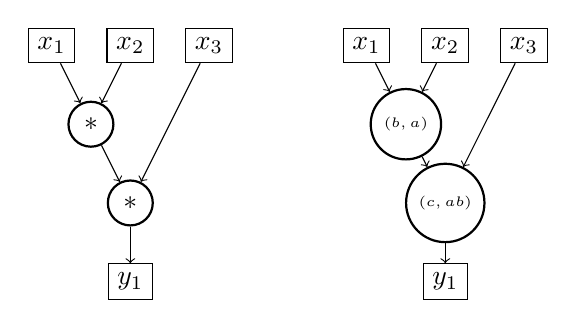
\begin{tikzpicture}
    \tikzstyle{node}=[circle,thick,draw=black,minimum size=4mm]
    \tikzstyle{arg}=[rectangle,thin,draw=black,minimum size=4mm]
    
    \begin{scope}
      \node[arg](in1){$x_1$};
      \node[arg,right of=in1](in2){$x_2$};
      \node[arg,right of=in2](in3){$x_3$};
      \node[node,below of=in1,xshift=5mm](times1){$*$};
      \node[node,below of=times1,xshift=5mm](times2){$*$};
      \node[arg,below of=times2](out){$y_1$};

      \path[->]
      (in1) edge (times1)
      (in2) edge (times1)
      (times1) edge (times2)
      (in3) edge (times2)
      (times2) edge (out);
    \end{scope}

    \begin{scope}[xshift=4cm]
      \node[arg](in1){$x_1$};
      \node[arg,right of=in1](in2){$x_2$};
      \node[arg,right of=in2](in3){$x_3$};
      \node[node,below of=in1,xshift=5mm](times1){\tiny$(b,a)$};
      \node[node,below of=times1,xshift=5mm](times2){\tiny$(c,ab)$};
      \node[arg,below of=times2](out){$y_1$};

      \path[->]
      (in1) edge (times1)
      (in2) edge (times1)
      (times1) edge (times2)
      (in3) edge (times2)
      (times2) edge (out);
    \end{scope}
  \end{tikzpicture}
  \caption{A circuit and its derivative at the point $x=(a,b,c)$.}
  \label{fig:derivative}
\end{figure}

Taking the derivative of a circuit at $x$ amounts to chose for each
node the best linear approximation at the point where it is
evaluated. It is clear that this yields the best linear approximation
for the circuit at $x$.

\begin{proposition}
  $\eval_{\diff_xC}=J_{\eval_C}(x)$.
\end{proposition}

It is also clear that $\diff_xC$ is defined over a basis that is
exclusively made of matrices with coefficients in $\R$, in other words
$\diff_xC$ is defined in $RMod{\R}$. We have thus defined a
transformation from black-box derivable functions to black-box
matrices.

Now the black-box $\diff_xC$ can be queried by black-box algorithms to
obtain information about the Jacobian. The most simple application is
to compute the directional derivative in $x$ along a direction $u$:
for this task it suffices to evaluate the circuit once since
$\eval_{\diff_xC}(u)$ is the desired value. Computing the derivative
along $n$ linearly independent directions yields the whole Jacobian
and this corresponds to the direct mode in automatic
differentiation\footnote{To be more precise, direct mode automatic
  differentiation constructs $\diff_xC$ and evaluates the $n$
  directions in parallel, thus reducing the amount of storage
  needed.}.

When the circuit has many inputs but only one output, there is a more
convenient way to get the whole gradient with only one black-box
query: $\diff_xC$ computes a linear form whose coefficients are
exactly the coefficients of the gradient, thus the dual circuit
$\dual{(\diff_xC)}$ computes the transposed form\footnote{We haven't
  actually proven the transposition theorem for an arbitrary basis,
  but it should be clear how to generalize it.}, or column vector. The
single query $\eval_{\dual{(\diff_xC)}}(1)$ yields this vector. This
is exactly what is called ``reverse mode'' in automatic
differentiation.

Note however that one is not limited to direct or reverse mode: any
black-box algorithm can be combined with the derivative circuit to
obtain information on the original function. For example Wiedemann's
algorithm \cite{Wie86} can be used to determine if the function is
invertible around $x$ and directional derivatives of the inverse can
be computed.

Of course, direct and reverse automatic differentiation can be defined
by the more classical chain rule, and then the transposition theorem
can be derived as a special case of the reverse mode by observing
that, when all the nodes of the circuit are linear maps, $C=\diff_xC$
for any $x$. After all, the code transformation techniques given in
\cite{BoLeSc03} and further developed in Section \ref{sec:} were
already invented by researchers in AD \cite{GVM91}, though not often
implemented. 

This being said, why treat transposition separately?  The answer is
manifold and we only list here some key points.
\begin{itemize}
\item AD is often interested in recovering the full Jacobian, instead
  of just having a black-box for it. For an $n\times m$ matrix, this
  requires $n$ queries in direct mode or $m$ queries in reverse
  mode. In both cases, AD tools do more work than what we would like
  to.
\item Many AD tools do not optimize the computation of $\diff_xC$ for
  the case where nodes are linear and still compute the whole
  circuit. In particular, many AD tools generate a graph
  representation of an arithmetic circuit from a program instead of
  directly transposing the code. This adds a constant overhead to the
  case of transposition where simply $\diff_xC=C$.
\item If the circuit $\diff_xC$ is computed, it must be fully stored
  in memory for reverse mode. This may seem innocuous as $\diff_xC$
  has the same size as $C$, but consider programs that compute
  $\eval_C$ by means of for loops or other iterative constructs: while
  the evaluation of $C$ is compact and cheap, the evaluation of
  $\diff_xC$ possibly requires to introduce a new variable for each
  iteration of the loop. Depending on the implementation, this may
  lead to code or storage bloat. In the case of transposition, this
  never happens since for loops are directly reversed (at least when
  all the variables are linear). Griewank \cite{Gri92} gives a
  time/memory compromise that permits to keep both storage and time in
  a factor of $\log n$ from the original program, but this is still
  not as good as transposition.
\item Our approach is more general in that it permits to automatically
  treat functions that depend both on linear and non-linear arguments
  without any help from the user. Thanks to this, we are able to treat
  recursive functions, while, to the extent of our knowledge, no AD
  tool can.
\item Our approach is algebraic and permits to prove bounds on the
  algebraic complexity of the generated programs, while AD tools
  usually only deal with floating point numbers. More generally, AD
  languages are usually less rich than \tAL.
\end{itemize}




% Local Variables:
% mode:flyspell
% ispell-local-dictionary:"american"
% mode:TeX-PDF
% mode:reftex
% TeX-master: "../these"
% End:
%

\chapter{Linearity inference of karatsuba multiplication}
\label{cha:line-infer-karats}
\lstset{language=haskell}

\begin{lstlisting}
data L = L Integer
data S = S Integer

class Ring r where
  zero :: r
  (<+>) :: r -> r -> r
  (<*>) :: r -> S -> r
  neg :: r -> r
  
class Ring r => Module m r | m -> r where
  zeroM :: m
  (<<*) :: m -> S -> m
  (>>>) :: m -> Integer -> r
  (<<<) :: r -> Integer -> m
  (<++>) :: m -> m -> m
  add :: m -> m -> Integer -> m
  add a b n = foldl (<++>) zeroM 
              [((a>>>i) <+> (b>>>i))<<<i | i <- [1..n]]
  
instance Ring L where
  zero = L 0
  (L x) <+> (L y) = L (x+y)
  (L x) <*> (S y) = L (x*y)
  neg (L x) = L (-x)
  
instance Ring S where
  zero = S 0
  (S x) <+> (S y) = S (x+y)  
  (S x) <*> (S y) = S (x*y)
  neg (S x) = S (-x)

one = S 1

instance Ring r => Module [r] r where
  zeroM = [zero]
  [] <<* x = []
  (x:xs) <<* y = (x <*> y):(xs <<* y)
  [] >>> i = zero
  (x:xs) >>> i =
    if i < 1 then zero else if i == 1 then x else xs >>> (i-1)
  x <<< i = if i <= 1 then [x] else zero:(x <<< (i-1))
  [] <++> [] = []
  (x:xs) <++> [] = x:(xs <++> [])
  [] <++> (y:ys) = y:([] <++> ys)
  (x:xs) <++> (y:ys) = (x <+> y):(xs <++> ys)
  add [] [] n = []
  add [] (y:ys) n =
    if n > 0 then y:(add [] ys (n-1)) else []
  add (x:xs) [] n =
    if n > 0 then x:(add xs [] (n-1)) else []
  add (x:xs) (y:ys) n =
    if n > 0 then (x<+>y):(add xs ys (n-1)) else []


-- Karatsuba multiplication : the system will infer
-- shift :: Ring r => [r] -> Integer -> [r]
-- split :: Ring r => [r] -> Integer -> ([r], [r])
-- kara :: Ring r => [r] -> [S] -> Integer -> [r]

shift x n = if n <= 0 then x else shift (zero:x) (n-1)

split [] n = ([], [])
split (x:xs) n =
  if n <= 0
  then ([], x:xs)
  else let (a, b) = split xs (n-1) in (x:a, b)

kara [] y n = []
kara x [] n = []
kara x y n =
  if n <= 0
  then []
  else if n == 1 
       then [(x!!0) <*> (y!!0)]
       else 
         let h = n `div` 2 in
         let (a0, a1) = split x h in
         let (b0, b1) = split y h in
         let x0 = kara a0 b0 h in
         let x2 = kara a1 b1 (n-h) in
         let xx1 = kara (a1 <++> a0) (b1 <++> b0) (n-h) in
         let x1 = xx1 <++> ((x0 <++> x2) <<* (neg one)) in
         (shift x2 n) <++> (shift x1 h) <++> x0
\end{lstlisting}                    
                  

% Local Variables:
% mode:flyspell
% ispell-local-dictionary:"american"
% mode:TeX-PDF
% mode:reftex
% TeX-master: "../these"
% End:
%




%%% Local Variables: 
%%% mode:flyspell
%%% ispell-local-dictionary:"american"
%%% mode: TeX-PDF
%%% mode: reftex
%%% TeX-master: "../these"
%%% End: 
